\documentclass[10pt,ignorenonframetext,]{beamer}
\setbeamertemplate{caption}[numbered]
\setbeamertemplate{caption label separator}{: }
\setbeamercolor{caption name}{fg=normal text.fg}
\beamertemplatenavigationsymbolsempty
\usepackage{lmodern}
\usepackage{amssymb,amsmath}
\usepackage{ifxetex,ifluatex}
\usepackage{fixltx2e} % provides \textsubscript
\ifnum 0\ifxetex 1\fi\ifluatex 1\fi=0 % if pdftex
  \usepackage[T1]{fontenc}
  \usepackage[utf8]{inputenc}
\else % if luatex or xelatex
  \ifxetex
    \usepackage{mathspec}
  \else
    \usepackage{fontspec}
  \fi
  \defaultfontfeatures{Ligatures=TeX,Scale=MatchLowercase}
\fi
\usetheme[]{Singapore}
\usefonttheme{serif}
% use upquote if available, for straight quotes in verbatim environments
\IfFileExists{upquote.sty}{\usepackage{upquote}}{}
% use microtype if available
\IfFileExists{microtype.sty}{%
\usepackage{microtype}
\UseMicrotypeSet[protrusion]{basicmath} % disable protrusion for tt fonts
}{}
\newif\ifbibliography
\hypersetup{
            pdftitle={Module 8: Tree-based Methods},
            pdfauthor={Stefanie Muff, Department of Mathematical Sciences, NTNU},
            colorlinks=true,
            linkcolor=Maroon,
            citecolor=Blue,
            urlcolor=blue,
            breaklinks=true}
\urlstyle{same}  % don't use monospace font for urls
\usepackage{color}
\usepackage{fancyvrb}
\newcommand{\VerbBar}{|}
\newcommand{\VERB}{\Verb[commandchars=\\\{\}]}
\DefineVerbatimEnvironment{Highlighting}{Verbatim}{commandchars=\\\{\}}
% Add ',fontsize=\small' for more characters per line
\usepackage{framed}
\definecolor{shadecolor}{RGB}{248,248,248}
\newenvironment{Shaded}{\begin{snugshade}}{\end{snugshade}}
\newcommand{\KeywordTok}[1]{\textcolor[rgb]{0.13,0.29,0.53}{\textbf{#1}}}
\newcommand{\DataTypeTok}[1]{\textcolor[rgb]{0.13,0.29,0.53}{#1}}
\newcommand{\DecValTok}[1]{\textcolor[rgb]{0.00,0.00,0.81}{#1}}
\newcommand{\BaseNTok}[1]{\textcolor[rgb]{0.00,0.00,0.81}{#1}}
\newcommand{\FloatTok}[1]{\textcolor[rgb]{0.00,0.00,0.81}{#1}}
\newcommand{\ConstantTok}[1]{\textcolor[rgb]{0.00,0.00,0.00}{#1}}
\newcommand{\CharTok}[1]{\textcolor[rgb]{0.31,0.60,0.02}{#1}}
\newcommand{\SpecialCharTok}[1]{\textcolor[rgb]{0.00,0.00,0.00}{#1}}
\newcommand{\StringTok}[1]{\textcolor[rgb]{0.31,0.60,0.02}{#1}}
\newcommand{\VerbatimStringTok}[1]{\textcolor[rgb]{0.31,0.60,0.02}{#1}}
\newcommand{\SpecialStringTok}[1]{\textcolor[rgb]{0.31,0.60,0.02}{#1}}
\newcommand{\ImportTok}[1]{#1}
\newcommand{\CommentTok}[1]{\textcolor[rgb]{0.56,0.35,0.01}{\textit{#1}}}
\newcommand{\DocumentationTok}[1]{\textcolor[rgb]{0.56,0.35,0.01}{\textbf{\textit{#1}}}}
\newcommand{\AnnotationTok}[1]{\textcolor[rgb]{0.56,0.35,0.01}{\textbf{\textit{#1}}}}
\newcommand{\CommentVarTok}[1]{\textcolor[rgb]{0.56,0.35,0.01}{\textbf{\textit{#1}}}}
\newcommand{\OtherTok}[1]{\textcolor[rgb]{0.56,0.35,0.01}{#1}}
\newcommand{\FunctionTok}[1]{\textcolor[rgb]{0.00,0.00,0.00}{#1}}
\newcommand{\VariableTok}[1]{\textcolor[rgb]{0.00,0.00,0.00}{#1}}
\newcommand{\ControlFlowTok}[1]{\textcolor[rgb]{0.13,0.29,0.53}{\textbf{#1}}}
\newcommand{\OperatorTok}[1]{\textcolor[rgb]{0.81,0.36,0.00}{\textbf{#1}}}
\newcommand{\BuiltInTok}[1]{#1}
\newcommand{\ExtensionTok}[1]{#1}
\newcommand{\PreprocessorTok}[1]{\textcolor[rgb]{0.56,0.35,0.01}{\textit{#1}}}
\newcommand{\AttributeTok}[1]{\textcolor[rgb]{0.77,0.63,0.00}{#1}}
\newcommand{\RegionMarkerTok}[1]{#1}
\newcommand{\InformationTok}[1]{\textcolor[rgb]{0.56,0.35,0.01}{\textbf{\textit{#1}}}}
\newcommand{\WarningTok}[1]{\textcolor[rgb]{0.56,0.35,0.01}{\textbf{\textit{#1}}}}
\newcommand{\AlertTok}[1]{\textcolor[rgb]{0.94,0.16,0.16}{#1}}
\newcommand{\ErrorTok}[1]{\textcolor[rgb]{0.64,0.00,0.00}{\textbf{#1}}}
\newcommand{\NormalTok}[1]{#1}
\usepackage{graphicx,grffile}
\makeatletter
\def\maxwidth{\ifdim\Gin@nat@width>\linewidth\linewidth\else\Gin@nat@width\fi}
\def\maxheight{\ifdim\Gin@nat@height>\textheight0.8\textheight\else\Gin@nat@height\fi}
\makeatother
% Scale images if necessary, so that they will not overflow the page
% margins by default, and it is still possible to overwrite the defaults
% using explicit options in \includegraphics[width, height, ...]{}
\setkeys{Gin}{width=\maxwidth,height=\maxheight,keepaspectratio}

% Prevent slide breaks in the middle of a paragraph:
\widowpenalties 1 10000
\raggedbottom

\AtBeginPart{
  \let\insertpartnumber\relax
  \let\partname\relax
  \frame{\partpage}
}
\AtBeginSection{
  \ifbibliography
  \else
    \let\insertsectionnumber\relax
    \let\sectionname\relax
    \frame{\sectionpage}
  \fi
}
\AtBeginSubsection{
  \let\insertsubsectionnumber\relax
  \let\subsectionname\relax
  \frame{\subsectionpage}
}

\setlength{\parindent}{0pt}
\setlength{\parskip}{6pt plus 2pt minus 1pt}
\setlength{\emergencystretch}{3em}  % prevent overfull lines
\providecommand{\tightlist}{%
  \setlength{\itemsep}{0pt}\setlength{\parskip}{0pt}}
\setcounter{secnumdepth}{0}
\usepackage{multirow}

\title{Module 8: Tree-based Methods}
\subtitle{TMA4268 Statistical Learning V2020}
\author{Stefanie Muff, Department of Mathematical Sciences, NTNU}
\date{February 28 and March 2, 2020}

\begin{document}
\frame{\titlepage}

\begin{frame}

Last update: February 25, 2020

\end{frame}

\begin{frame}{Acknowledgements}

\begin{itemize}
\item
  A lot of this material stems from Mette Langaas and her TAs (in
  particular Thea Roksv\aa g, who developed the set of slides, but also
  Mette Langaas and Julia Debik). Thanks to Mette for the permission to
  use the material!
\item
  Some of the figures and slides in this presentation are taken (or are
  inspired) from James et al. (2013).
\end{itemize}

\end{frame}

\begin{frame}{Introduction}

\begin{block}{Learning material for this module}

\vspace{2mm}

\begin{itemize}
\tightlist
\item
  James et al (2013): An Introduction to Statistical Learning. Chapter
  8.\\
\item
  All the material presented on these module slides.
\end{itemize}

\end{block}

\end{frame}

\begin{frame}

\begin{block}{What will you learn?}

\vspace{2mm}

You will get to know

\begin{itemize}
\tightlist
\item
  Decision trees

  \begin{itemize}
  \tightlist
  \item
    Regression trees\\
  \item
    Classification trees\\
  \end{itemize}
\item
  Pruning a tree
\item
  Bagging
\item
  Variable importance
\item
  Random forests
\item
  Boosting
\end{itemize}

and learn how to apply all that.

\end{block}

\end{frame}

\begin{frame}[fragile]

\begin{block}{Example 1 (from chapter 8.1; \texttt{Hitters} data)}

\vspace{1mm}

\begin{itemize}
\item
  Baseball players' salaries may depend on their experience (in years)
  and the number of hits.
\item
  High salaries (yellow, red) vs low salaries (blue, green), salaries
  given on \(\log\)-scale. How can these be stratified for prediction of
  the salary?
\end{itemize}

\centering
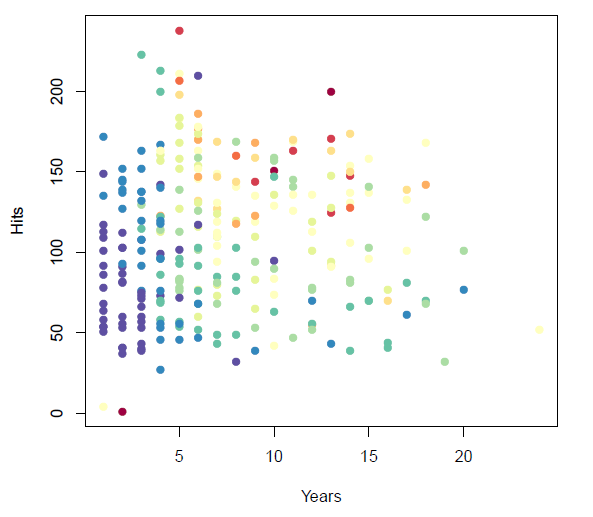
\includegraphics[width=0.60000\textwidth]{hits.png}

\end{block}

\end{frame}

\begin{frame}

\begin{block}{Main idea of tree-based methods}

\vspace{2mm}

\begin{itemize}
\item
  Divide the area into rectangles with similar salaries.
\item
  Idea: Derive a set of decision (splitting) rules for segmenting the
  predictor space into a number of finer and finer regions.
\item
  All points in the same region will be given the same predictive value
  (the mean of all values in that square, or a majority vote).
\end{itemize}

Visualisaztion in two dimensions:

\centering
\includegraphics[width=0.50000\textwidth]{../../ISLR/Figures/Chapter8/8.2.png}

\end{block}

\end{frame}

\begin{frame}

The series of splitting rules can be visualized with a \emph{regression
tree}.

The following tree (which corresponds to the split in the previous
slide) has three \emph{leafs} (terminal nodes), and two \emph{internal
nodes}:

\(~\)

\centering

\includegraphics[width=0.50000\textwidth]{../../ISLR/Figures/Chapter8/8.1.png}

\end{frame}

\begin{frame}

\begin{block}{More than two predictors?}

\vspace{2mm}

\begin{itemize}
\item
  With more than two predictors we cannot draw the partition of the data
  in a coordinate system, but we can still draw the regression tree.
\item
  Before we discuss how the algorithm splits the data into regions, let
  us look at a somewhat more interesting example.
\end{itemize}

\end{block}

\end{frame}

\begin{frame}

\begin{block}{Example 2: Detection of Minor Head Injury}

\tiny
(Artificial data) \vspace{2mm}

\normalsize

\begin{itemize}
\item
  Data from patients that enter hospital. The aim is to quickly assess
  whether a patient as a brain injury or not (binary outcome =
  classification problem).
\item
  Patients are investigated and (possible) asked questions.
\item
  Our job: To build a good model to predict quickly if someone has a
  brain injury. The method should be

  \begin{itemize}
  \item
    \textbf{easy} to interpret for the medical personell that are not
    skilled in statistics, and
  \item
    \textbf{fast}, such that the medical personell quickly can identify
    a patient that needs treatment.
  \end{itemize}
\end{itemize}

\(\rightarrow\) This can be done by using tree-based methods.

\vspace{4mm}

\small
Note: Of course, the model should be built \emph{before} a new emergency
patient arrives, using data that is already available.

\end{block}

\end{frame}

\begin{frame}[fragile]

The dataset includes data about 1321 patients and is a modified and
smaller version of the (simulated) dataset \texttt{headInjury} from the
\texttt{DAAG} library.

\footnotesize

\begin{verbatim}
##    amnesia bskullf GCSdecr GCS.13 GCS.15 risk consc oskullf vomit
## 3        0       0       0      0      0    0     0       0     0
## 9        0       0       0      0      0    1     0       0     0
## 11       0       0       0      0      0    0     0       0     0
## 12       1       0       0      0      0    0     0       0     0
## 14       0       0       0      0      0    0     0       0     0
## 16       0       0       0      0      0    0     0       0     0
##    brain.injury age
## 3             0  44
## 9             0  67
## 11            0  62
## 12            0   1
## 14            0  55
## 16            0  63
\end{verbatim}

\normalsize

\end{frame}

\begin{frame}[fragile]

\begin{itemize}
\tightlist
\item
  The variable \texttt{brain.injury} will be the response of our model
  (=1 if a person has an acute brain injury, =0 otherwise).
\end{itemize}

\vspace{0mm}

\begin{itemize}
\tightlist
\item
  250 (19\%) of the patients have a clinically important brain injury.
\end{itemize}

\vspace{0mm}

\begin{itemize}
\item
  The 10 variables used as explanatory variables describe the state of
  the patient, for example

  \begin{itemize}
  \tightlist
  \item
    Is he/she vomiting?
  \item
    Is the Glasgow Coma Scale (GCS)
    score\footnote{The GCS scale goes back to an article in the Lancet in 1974, and is used to describe the level of consciousness of patients with an acute brain injury. See <https://www.glasgowcomascale.org/what-is-gcs/>}
    after 2 hours equal to 15 (or not)?
  \item
    Has he/she an open scull fracture?
  \item
    Has he/she had a loss of consciousness?
  \item
    and so on.
  \end{itemize}
\end{itemize}

\end{frame}

\begin{frame}

The classification tree made from a training set of 850 randomly drawn
observations (training set) for the head injury example looks like this:

\begin{center}\includegraphics[width=0.7\linewidth]{8Trees_files/figure-beamer/injury1-1} \end{center}

\small
Note: The split criterion at each node is to the left. For example,
``GCS.15:0'' means that ``GCS.15=0'' goes left, and ``GCS.15=1'' goes
right.

\end{frame}

\begin{frame}[fragile]

\footnotesize

\begin{Shaded}
\begin{Highlighting}[]
\KeywordTok{print}\NormalTok{(headtree)}
\end{Highlighting}
\end{Shaded}

\begin{verbatim}
## node), split, n, deviance, yval, (yprob)
##       * denotes terminal node
## 
##  1) root 850 819.00 0 ( 0.8129 0.1871 )  
##    2) GCS.15: 0 711 520.00 0 ( 0.8805 0.1195 )  
##      4) bskullf: 0 663 398.00 0 ( 0.9110 0.0890 )  
##        8) risk: 0 487 203.00 0 ( 0.9466 0.0534 )  
##         16) age < 68.5 445 131.00 0 ( 0.9663 0.0337 ) *
##         17) age > 68.5 42  48.30 0 ( 0.7381 0.2619 ) *
##        9) risk: 1 176 170.00 0 ( 0.8125 0.1875 ) *
##      5) bskullf: 1 48  66.20 1 ( 0.4583 0.5417 )  
##       10) age < 42.5 13  11.20 0 ( 0.8462 0.1538 ) *
##       11) age > 42.5 35  43.60 1 ( 0.3143 0.6857 ) *
##    3) GCS.15: 1 139 192.00 1 ( 0.4676 0.5324 )  
##      6) GCS.13: 0 121 167.00 0 ( 0.5289 0.4711 )  
##       12) risk: 0 78 101.00 0 ( 0.6538 0.3462 )  
##         24) age < 66.5 66  77.30 0 ( 0.7273 0.2727 ) *
##         25) age > 66.5 12  13.50 1 ( 0.2500 0.7500 ) *
##       13) risk: 1 43  52.70 1 ( 0.3023 0.6977 ) *
##      7) GCS.13: 1 18   7.72 1 ( 0.0556 0.9444 ) *
\end{verbatim}

\normalsize

\end{frame}

\begin{frame}

\begin{itemize}
\item
  By using simple decision rules related to the most important
  explanatory variables the medical staff can now assess the probability
  of a brain injury.
\item
  The decision can go ``top down'', because the most informative
  predictors are usually split first.
\item
  Example: The staff might check if the Glasgow Coma Scale of the
  patient is 15 after 2h, and if it was 13 at the beginning. In that
  case, the probability of brain injury is estimated to be 0.944 (node 7
  in printout).
\end{itemize}

\textbf{Advantages}:

\begin{itemize}
\item
  Decision trees are easier to interpret than many of the classification
  (and regression) methods that we have studied so far.
\item
  Decision trees provide an easy way to visualize the data for
  non-statisticians.
\end{itemize}

\end{frame}

\begin{frame}

\begin{block}{Some terminology}

\begin{itemize}
\item
  CARTs (Classification and regression trees) are usually drawn upside
  down, where the top node is called the \emph{root}.
\item
  The \emph{terminal nodes} or \emph{leaf nodes} are the nodes at the
  bottom. These are written symbolically as \(R_j\) for
  \(j = 1, 2, ..., J\)
\item
  The \(R_j\) will be referred to as \emph{non-overlapping regions} and
  are high-dimensional rectangles (boxes).
\item
  \emph{Internal nodes} are all nodes between the root and the terminal
  nodes. These nodes correspond to the partitions of the predictor
  space.
\item
  \emph{Branches}: segment of the tree connecting the nodes.
\end{itemize}

\vspace{2mm} We will consider only binary splits on one variable, but
multiway splits and linear combination of variabes are possible - but
not so common.

\end{block}

\end{frame}

\begin{frame}{Regression tree (continous outcome)}

Assume that we have a dataset consisting of \(n\) pairs
\((\boldsymbol{x}_i,y_i)\), \(i=1,\ldots,n\), and each predictor is
\({\boldsymbol{x}}_i=(x_{i1},x_{i2},...,x_{ip})\). The aim is to predict
\(y_i\).

\vspace{2mm} Two steps:

\begin{enumerate}
\def\labelenumi{\arabic{enumi}.}
\item
  Divide the predictor space into non-overlapping regions
  \(R_1,R_2,\ldots,R_J\).
\item
  For every observation that falls into region \(R_j\) we make the same
  prediction - which is the mean of the responses for the training
  observations that fall into \(R_j\).
\end{enumerate}

\vspace{2mm}

\textbf{But}: How to divide the predictor space into non-overlapping
regions \(R_1,R_2,\ldots,R_J\)?

\end{frame}

\begin{frame}

We could try to minimize the RSS (residual sums of squares) on the
training set given by

\[
\text{RSS}=\sum_{j=1}^J \sum_{i \in R_j}(y_i-\hat{y}_{R_j})^2,
\]

where \(\hat{y}_{R_j}\) is the mean response for the training
observations in region \(j\). The mean \(\hat{y}_{R_j}\) is also the
predicted value for a new observations that falls into region \(j\).

To do this we need to consider every partition of the predictor space,
and compute the RSS for each partition.

\textbf{But}: An exhaustive search over possible splits is
\emph{computationally infeasible}!
\footnote{In fact, constructing optimal binary decision trees is an NP-complete problem (Hyafil and Rivest, 1976).}

\end{frame}

\begin{frame}

\begin{block}{Recursive binary splitting}

\vspace{2mm}

\begin{itemize}
\item
  A \emph{greedy} approach is taken (aka top-down) - called
  \emph{recursive binary splitting}: Find a split that minimizes RSS at
  each
  step\footnote{This does not necessarily give the optimal global solution, but will give the best solution at each split, given what is done previously.}.
\item
  We start at the top of the tree and divide the predictor space into
  two regions, \(R_1\) and \(R_2\) by making a decision rule for one of
  the predictors \(x_1, x_2,...,x_p\). If we define the two regions by
  \(R_1(j,s)=\{x \mid x_j<s\}\) and \(R_2(j,s)=\{x \mid x_j\geq s\}\),
  it means that we need to find the (predictor) \(j\) and (splitting
  point) \(s\) that minimize
  \[\sum_{i: x_i \in R_1(j,s)}(y_i-\hat{y}_{R_1})^2+\sum_{i: x_i \in R_2(j,s)}(y_i -\hat{y}_{R_2})^2 \ ,\]
  where \(\hat{y}_{R_1}\) and \(\hat{y}_{R_2}\) are the mean responses
  for the training observations in \(R_1(j,s)\) and \(R_2(j,s)\)
  respectively. This way we get the two first branches in our decision
  tree.
\end{itemize}

\end{block}

\end{frame}

\begin{frame}

\begin{itemize}
\item
  We repeat the process to make branches further down in the tree.
\item
  For every iteration we let each single split depend on \emph{only one
  of the predictors}, giving us two new branches.
\item
  This is done \emph{successively} and in each step we choose the split
  that gives the
  \emph{\textcolor{red}{best split at that particular step}},
  \emph{i.e.,} the split that gives the smallest RSS.
\item
  However, this time, instead of splitting the entire predictor space,
  we split only
  \emph{\textcolor{red}{one of the previously identified regions}}.
\item
  Continue splitting the predictor space until we reach some
  \emph{stopping criterion}. For example we stop when a region contains
  less than 10 observations or when the reduction in the RSS is smaller
  than a specified limit.
\end{itemize}

\vspace{1mm}

\textbf{Q}: Why is this algorithm called \emph{greedy}?

\end{frame}

\begin{frame}[fragile]

\begin{block}{Regression tree: ozone example}

\vspace{2mm}

Consider the \texttt{ozone} data set from the \texttt{ElemStatLearn}
library. The data set consists of 111 observations on the following
variables:

\begin{itemize}
\tightlist
\item
  \texttt{ozone} : the concentration of ozone in ppb
\item
  \texttt{radiation}: the solar radiation (langleys)
\item
  \texttt{temperature} : the daily maximum temperature in degrees F
\item
  \texttt{wind} : wind speed in mph
\end{itemize}

\vspace{2mm}

\scriptsize

\begin{Shaded}
\begin{Highlighting}[]
\KeywordTok{head}\NormalTok{(myozone)}
\end{Highlighting}
\end{Shaded}

\begin{verbatim}
##   ozone radi temp wind
## 1    41  190   67  7.4
## 2    36  118   72  8.0
## 3    12  149   74 12.6
## 4    18  313   62 11.5
## 5    23  299   65  8.6
## 6    19   99   59 13.8
\end{verbatim}

\end{block}

\end{frame}

\begin{frame}[fragile]

Let's fit a regression tree with \texttt{ozone} as our response variable
and \texttt{temperature} and \texttt{wind} as predictors.

\scriptsize

\begin{Shaded}
\begin{Highlighting}[]
\NormalTok{ozone.trainID =}\StringTok{ }\KeywordTok{sample}\NormalTok{(}\DecValTok{1}\OperatorTok{:}\DecValTok{111}\NormalTok{, }\DecValTok{75}\NormalTok{)}
\NormalTok{ozone.train =}\StringTok{ }\NormalTok{myozone[ozone.trainID, ]}
\NormalTok{ozone.test =}\StringTok{ }\NormalTok{myozone[}\OperatorTok{-}\NormalTok{ozone.trainID, ]}
\end{Highlighting}
\end{Shaded}

\normalsize
Use the default settings in the tree function: \scriptsize

\begin{Shaded}
\begin{Highlighting}[]
\NormalTok{ozone.tree =}\StringTok{ }\KeywordTok{tree}\NormalTok{(ozone }\OperatorTok{~}\StringTok{ }\NormalTok{temp }\OperatorTok{+}\StringTok{ }\NormalTok{wind, }\DataTypeTok{data =}\NormalTok{ ozone.train)}
\end{Highlighting}
\end{Shaded}

\begin{center}\includegraphics[width=0.6\linewidth]{8Trees_files/figure-beamer/ozone1-1} \end{center}

\end{frame}

\begin{frame}[fragile]

\begin{itemize}
\item
  We see that \texttt{temperature} is the ``most important'' predictor
  for predicting the ozone concentration. Observe that we can split on
  the same variable several times.
\item
  Focus on the regions \(R_j\), \(j=1,\ldots, J\). What is \(J\) here?
\end{itemize}

\end{frame}

\begin{frame}

\begin{block}{Tree- vs region plot}

\vspace{2mm}

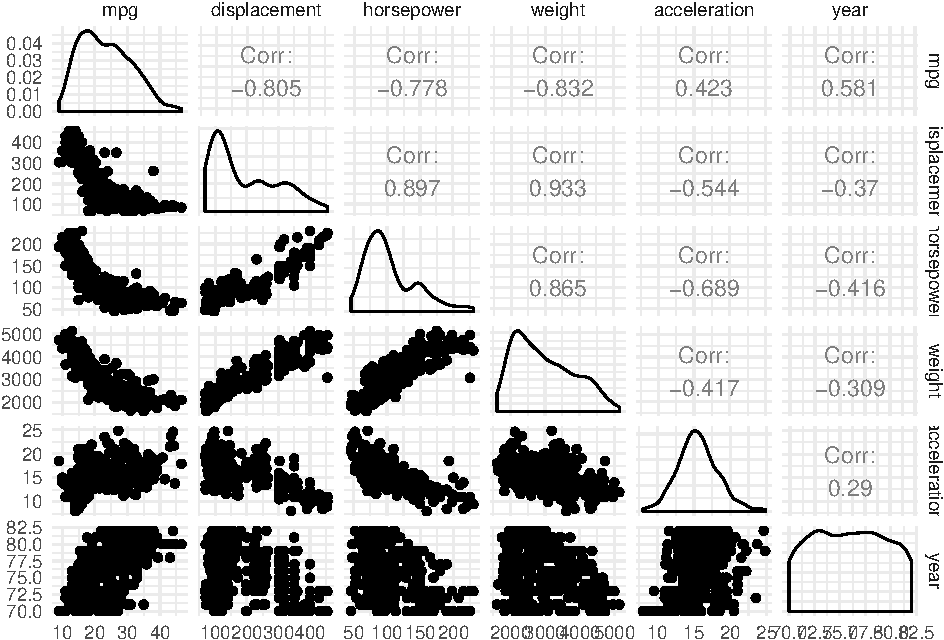
\includegraphics{8Trees_files/figure-beamer/unnamed-chunk-7-1.pdf}

\vspace{-2mm} \textbf{Q}:

\begin{itemize}
\tightlist
\item
  Explain the connection between the tree and the region plot.
\item
  Advantages and disadvantages of letting each single split depend on
  only one of the predictors?
\item
  Does our tree include interactions between variables?
\end{itemize}

\end{block}

\end{frame}

\begin{frame}[fragile]

\begin{block}{R: function \texttt{tree} in library \texttt{tree}}

\vspace{2mm}

\begin{itemize}
\item
  R package \texttt{tree} by Brian D. Ripley (B. Ripley 2019).
\item
  You get information about the function when you type \texttt{?tree}
  into the \texttt{R} console.
\item
  Note: The default choice for a function to minimize is the deviance,
  and for normal data (as we may assume for regression), the deviance is
  proportional to the RSS.
\end{itemize}

\begin{itemize}
\tightlist
\item
  A competing R function is \texttt{rpart}, explained in
  \url{https://cran.r-project.org/web/packages/rpart/vignettes/longintro.pdf}
\end{itemize}

\end{block}

\end{frame}

\begin{frame}[fragile]

\begin{block}{Stopping criterion}

\vspace{2mm}

\begin{itemize}
\item
  When building the tree, we can (in principle) split until each leaf
  corresponds to one data point.
\item
  Usually we use a less stringent stopping criterion, like the minimal
  number of nodes per region and/or the minimum reduction in the RSS.
\item
  For example, the default in \texttt{tree()}: is given by
  \texttt{mincut=5,\ minsize=10,\ mindev=0.01}, thus a minimal size of 5
  nodes, the smallest nodes that are potentially split is 10, and the
  minimal reduction in deviance (RSS) equal to 0.01.
\item
  We could make the ozone tree much deeper by decreasing the minimal
  size of a region and chanding the minimum reduction in RSS:
\end{itemize}

\scriptsize

\begin{Shaded}
\begin{Highlighting}[]
\NormalTok{ozone.tree2 =}\StringTok{ }\KeywordTok{tree}\NormalTok{(ozone }\OperatorTok{~}\StringTok{ }\NormalTok{temp }\OperatorTok{+}\StringTok{ }\NormalTok{wind, }\DataTypeTok{data =}\NormalTok{ ozone.train, }\DataTypeTok{control =} \KeywordTok{tree.control}\NormalTok{(}\DecValTok{75}\NormalTok{, }
    \DataTypeTok{mincut =} \DecValTok{2}\NormalTok{, }\DataTypeTok{minsize =} \DecValTok{4}\NormalTok{, }\DataTypeTok{mindev =} \FloatTok{0.001}\NormalTok{))}
\end{Highlighting}
\end{Shaded}

\end{block}

\end{frame}

\begin{frame}

With the above command, the tree would become very fine. Overfitting?

\begin{center}\includegraphics[width=0.7\linewidth]{8Trees_files/figure-beamer/ozone2-1} \end{center}

\end{frame}

\begin{frame}[fragile]

\begin{block}{Tree performance}

\vspace{2mm}

\begin{itemize}
\tightlist
\item
  Test the predictive performance of our regression tree by using a
  training and a test set.
\item
  For the two trees (the shallow and the deep one from above), we get
  the following test MSEs:
\end{itemize}

\scriptsize

\begin{Shaded}
\begin{Highlighting}[]
\NormalTok{ozone.pred =}\StringTok{ }\KeywordTok{predict}\NormalTok{(ozone.tree, }\DataTypeTok{newdata =}\NormalTok{ ozone.test)}
\NormalTok{ozone.MSE =}\StringTok{ }\KeywordTok{mean}\NormalTok{((ozone.pred }\OperatorTok{-}\StringTok{ }\NormalTok{ozone.test}\OperatorTok{$}\NormalTok{ozone)}\OperatorTok{^}\DecValTok{2}\NormalTok{)}
\NormalTok{ozone.MSE}
\end{Highlighting}
\end{Shaded}

\begin{verbatim}
## [1] 384.4906
\end{verbatim}

\begin{Shaded}
\begin{Highlighting}[]
\NormalTok{ozone.pred2 =}\StringTok{ }\KeywordTok{predict}\NormalTok{(ozone.tree2, }\DataTypeTok{newdata =}\NormalTok{ ozone.test)}
\NormalTok{ozone.MSE2 =}\StringTok{ }\KeywordTok{mean}\NormalTok{((ozone.pred2 }\OperatorTok{-}\StringTok{ }\NormalTok{ozone.test}\OperatorTok{$}\NormalTok{ozone)}\OperatorTok{^}\DecValTok{2}\NormalTok{)}
\NormalTok{ozone.MSE2}
\end{Highlighting}
\end{Shaded}

\begin{verbatim}
## [1] 491.2656
\end{verbatim}

\vspace{1mm}

\normalsize
\emph{\textcolor{red}{How do we know if our tree performs good, or if there would be trees with a better predictive performance?}}

\end{block}

\end{frame}

\begin{frame}{Pruning}

\begin{itemize}
\item
  If we have a data set with many predictors or choose a stringent
  stopping criterion, we may fit a (too) large tree. Thus, the number of
  observations from the training set that falls into some of the regions
  \(R_j\) may be small \(\rightarrow\)
  \emph{\textcolor{red}{overfitting}}?
\item
  A smaller tree with fewer splits leads to fewer regions
  \(R_1, \ldots, R_J\) with more observations. This might lead to lower
  variance and better interpretation at the cost of more bias.
\item
  One possible alternative to the process described above is to grow the
  tree only so long as the decrease in the RSS due to each split exceeds
  some (high) threshold.
\item
  This strategy will result in smaller trees, but is
  \emph{\textcolor{red}{too short-sighted}}: a seemingly worthless split
  early on in the tree might be followed by a very good split --- that
  is, a split that leads to a large reduction in RSS later on.
\end{itemize}

\end{frame}

\begin{frame}

\begin{block}{Cost complexity pruning}

\begin{itemize}
\item
  Better idea: to grow a very large tree \(T_0\), and then
  \emph{\textcolor{red}{prune}} it back in order to obtain a
  \emph{\textcolor{red}{subtree}}.
\item
  \emph{\textcolor{red}{Cost complexity pruning}} is used for this: We
  try to find a subtree \(T\subset T_0\) that (for a given value of
  \(\alpha\)) minimizes \[
  C_{\alpha}(T)=Q(T)+\alpha |T|,
  \] where \(Q(T)\) is our cost function, \(|T|\) is the number of
  terminal nodes in tree \(T\). The parameter \(\alpha\) is then a
  parameter penalizing the number of terminal nodes, ensuring that the
  tree does not get too many branches.
\item
  For regression trees (continous outcome) we choose
  \[Q(T)=\sum_{m=1}^{|T|}\sum_{x_i\in R_m}(y_i - \hat{y}_{R_m})^2 \ .\]
\end{itemize}

\end{block}

\end{frame}

\begin{frame}

\begin{itemize}
\item
  For \(\alpha>0\) we get a pruned tree (note: the same pruned tree
  within a small range of \(\alpha\)).
\item
  For \(\alpha=0\) we get \(T_0\).
\item
  As \(\alpha\) increases we get shorter and shorter trees.
\end{itemize}

So, which value of \(\alpha\) is best?

\begin{itemize}
\item
  We can use \(K\)-fold cross-validation to find out!
\item
  Importantly, by increasing \(\alpha\), branches get pruned in a
  \emph{hierarchical (nested) fashion}.
\end{itemize}

Please study this
\href{https://www.math.ntnu.no/emner/TMA4268/2018v/notes/CART1MA87012017BoLindqvist.pdf}{note
from Bo Lindqvist in MA8701 in 2017 - Advanced topics in Statistical
Learning and Inference} for an example of how we perform cost complexity
pruning in detail. Alternatively, this method, with proofs, are given in
B. D. Ripley (1996), Section 7.2.

\end{frame}

\begin{frame}

\begin{block}{Building a regression tree: Algorithm 8.1}

\begin{enumerate}
\def\labelenumi{\arabic{enumi}.}
\item
  Use recursive binary splitting to grow a large tree on the training
  data, stopping only when each terminal node has fewer than some
  minimum number of observations.
\item
  Apply cost complexity pruning to the large tree in order to obtain a
  sequence of best subtrees, as a function of \(\alpha\).
\item
  Use \(K\)-fold cross-validation to choose \(\alpha\). That is, divide
  the training observations into \(k\) folds. For each
  \(k = 1,\ldots, K\):

  \begin{itemize}
  \tightlist
  \item
    Repeat Steps 1 and 2 on all but the \(k\)th fold of the training
    data.
  \item
    Evaluate the mean squared prediction error on the data in the
    left-out \(k\)th fold, as a function of \(\alpha\).
  \item
    Average the results for each value of \(\alpha\), and pick
    \(\alpha\) to minimize the average error.
  \end{itemize}
\item
  Return the subtree from Step 2 that corresponds to the chosen value of
  \(\alpha\).
\end{enumerate}

\end{block}

\end{frame}

\begin{frame}

\begin{block}{Pruning the ozone tree}

Let us start with the tree with many leaves, and then prune it with
5-fold CV. We can then plot the CV error as a function of tree size
(instead of \(\alpha\) -- why?):

\begin{center}\includegraphics[width=0.6\linewidth]{8Trees_files/figure-beamer/ozone.cv-1} \end{center}

Interestingly, it seems like a tree with 5 leaves performs best - which
corresponds to the original choice.

\end{block}

\end{frame}

\begin{frame}{Classification trees (binary or categorical outcome)}

\vspace{2mm}

\begin{itemize}
\tightlist
\item
  Remember the minor head injury example: Binary outcome (disease
  yes/no).
\end{itemize}

\vspace{1mm}

\begin{itemize}
\tightlist
\item
  Now allow for \(K\geq 2\) number of classes for the response.
\end{itemize}

\vspace{1mm}

\begin{itemize}
\tightlist
\item
  Building a decision tree in this setting is similar to building a
  regression tree for a quantitative response, but there are two main
  differences: \emph{the prediction} and \emph{the splitting criterion}.
\end{itemize}

\end{frame}

\begin{frame}

\textbf{1) The prediction:}

\begin{itemize}
\item
  In the regression case we use the mean value of the responses in
  \(R_j\) as a prediction for an observation that falls into region
  \(R_j\). \vspace{2mm}
\item
  For the \emph{\textcolor{red}{classification case}}, however, we have
  two possibilities:

  \begin{itemize}
  \tightlist
  \item
    \textbf{Majority vote}: Predict that the observation belongs to the
    most commonly occurring class of the training observations in
    \(R_j\).\\
  \item
    Estimate the \textbf{probability} that an observation \(x_i\)
    belongs to a class \(k\), \(\hat{p}_{jk}(x_i)\), and then classify
    according to a \textbf{threshold value}. This estimated probability
    is the proportion of class \(k\) training observations in region
    \(R_j\), with \(n_{jk}\) observations. Region \(j\) has \(N_j\)
    observations.
    \[\hat{p}_{jk} = \frac{1}{N_j} \sum_{i:x_i \in R_j} I(y_i = k)=\frac{n_{jk}}{N_j}.\]
  \end{itemize}
\end{itemize}

\end{frame}

\begin{frame}

\textbf{2) The splitting criterion:} We do not use RSS as a splitting
criterion for a qualitative variable. Instead we can use some
\emph{measure of impurity} of the node. For leaf node \(j\) and class
\(k=1,\ldots, K\):

\begin{itemize}
\tightlist
\item
  \textbf{Gini index}: \[
  G=\sum_{k=1}^K \hat{p}_{jk}(1-\hat{p}_{jk}) \ ,
  \] which is small if all of the \(\hat{p}_{jk}\)'s are close to 0 or
  1.
\end{itemize}

\vspace{1mm}

\begin{itemize}
\tightlist
\item
  \textbf{Cross entropy}: \[
  D=-\sum_{k=1}^K \hat{p}_{jk}\log\hat{p}_{jk} \ .
  \] Here \(\hat{p}_{jk}\) is the proportion of training observation in
  region \(j\) that are from class \(k\).
\end{itemize}

When making a split in our classification tree, we want to minimize the
Gini index or the cross-entropy.

\end{frame}

\begin{frame}

Why don't we just minimize the misclassification error
\[E= 1- \max_k{\hat{p}_{jk}} \ ?\]

\textbf{A}:

\begin{itemize}
\item
  The Gini index and Entropy are \emph{measure of impurity}. They are
  more sensitive to changes in the node probabilities.
\item
  Example for two classes: Assume we have two classes with 400 nodes
  each, written as \((400,400)\). Now we can choose between two splits:

  \begin{itemize}
  \tightlist
  \item
    Split 1: (100,300) and (300,100)\\
  \item
    Split 2: (200,400) and (200,0).
  \end{itemize}
\end{itemize}

Both splits result in 25\% misclassification. Which of these splits is
better? Probably the second one, because it produces a \emph{pure node}.

\end{frame}

\begin{frame}

\begin{itemize}
\tightlist
\item
  Moreover, The Gini index and Entropy are differentiable (preferred for
  numerical optimization!)
\end{itemize}

\begin{center}\includegraphics[width=0.6\linewidth]{8Trees_files/figure-beamer/purity-1} \end{center}

\end{frame}

\begin{frame}[fragile]

\begin{block}{Minor head injury - split with cross-entropy}

\vspace{1mm}

We use the 850 training samples to get a tree using cross-entropy
(deviance):

\scriptsize

\begin{Shaded}
\begin{Highlighting}[]
\NormalTok{tree.HIClass =}\StringTok{ }\KeywordTok{tree}\NormalTok{(brain.injury }\OperatorTok{~}\StringTok{ }\NormalTok{., }\DataTypeTok{data =}\NormalTok{ headInjury2, }\DataTypeTok{subset =}\NormalTok{ train, }
    \DataTypeTok{split =} \StringTok{"deviance"}\NormalTok{)}
\KeywordTok{summary}\NormalTok{(tree.HIClass)}
\end{Highlighting}
\end{Shaded}

\begin{verbatim}
## 
## Classification tree:
## tree(formula = brain.injury ~ ., data = headInjury2, subset = train, 
##     split = "deviance")
## Variables actually used in tree construction:
## [1] "GCS.15"  "bskullf" "risk"    "age"     "GCS.13" 
## Number of terminal nodes:  9 
## Residual mean deviance:  0.6604 = 555.4 / 841 
## Misclassification error rate: 0.1259 = 107 / 850
\end{verbatim}

\vspace{1mm} \textbf{Remark}: the deviance (\(-2\log(L)\)) is a scaled
version of the cross entropy:
\[-2\sum_{k=1}^K n_{jk} \log\hat{p}_{jk}\ , \text{where} \quad   \hat{p}_{jk}=\frac{n_{jk}}{N_j}\ , \]
thus \texttt{split="deviance"} implies that we split according to the
entropy criterion.

\end{block}

\end{frame}

\begin{frame}[fragile]

\scriptsize

\begin{Shaded}
\begin{Highlighting}[]
\KeywordTok{plot}\NormalTok{(tree.HIClass, }\DataTypeTok{type =} \StringTok{"proportional"}\NormalTok{)}
\KeywordTok{text}\NormalTok{(tree.HIClass, }\DataTypeTok{pretty =} \DecValTok{1}\NormalTok{)}
\end{Highlighting}
\end{Shaded}

\begin{center}\includegraphics[width=0.5\linewidth]{8Trees_files/figure-beamer/headInjury-1} \end{center}

\normalsize

\begin{itemize}
\item
  With \texttt{type="proportional"}, the length of branches are now
  proportional to the decrease in impurity.
\item
  The classification tree has two terminal nodes with factor ``0''
  originating from the same branch. Why do we get this ``unnecessary''
  split? (Hint: Node purity)
\end{itemize}

\end{frame}

\begin{frame}[fragile]

\begin{block}{Minor head injury - split with Gini index}

\vspace{2mm}

The same analysis with the Gini index:

\scriptsize

\begin{Shaded}
\begin{Highlighting}[]
\NormalTok{tree.HIClassG =}\StringTok{ }\KeywordTok{tree}\NormalTok{(brain.injury }\OperatorTok{~}\StringTok{ }\NormalTok{., headInjury2, }\DataTypeTok{subset =}\NormalTok{ train, }\DataTypeTok{split =} \StringTok{"gini"}\NormalTok{)}
\KeywordTok{summary}\NormalTok{(tree.HIClassG)}
\end{Highlighting}
\end{Shaded}

\begin{verbatim}
## 
## Classification tree:
## tree(formula = brain.injury ~ ., data = headInjury2, subset = train, 
##     split = "gini")
## Variables actually used in tree construction:
## [1] "GCS.15"  "bskullf" "risk"    "age"     "oskullf" "vomit"   "amnesia"
## [8] "consc"   "GCS.13" 
## Number of terminal nodes:  75 
## Residual mean deviance:  0.5202 = 403.2 / 775 
## Misclassification error rate: 0.1094 = 93 / 850
\end{verbatim}

\end{block}

\end{frame}

\begin{frame}[fragile]

\scriptsize

\begin{Shaded}
\begin{Highlighting}[]
\KeywordTok{plot}\NormalTok{(tree.HIClassG, }\DataTypeTok{type =} \StringTok{"proportional"}\NormalTok{)}
\KeywordTok{text}\NormalTok{(tree.HIClassG, }\DataTypeTok{pretty =} \DecValTok{1}\NormalTok{)}
\end{Highlighting}
\end{Shaded}

\begin{center}\includegraphics[width=0.7\linewidth]{8Trees_files/figure-beamer/headInjury2-1} \end{center}

\normalsize

This is a very bushy tree!

\end{frame}

\begin{frame}[fragile]

\begin{block}{Checking predictions}

\vspace{2mm}

We also use the classification tree to predict the status of the
patients in the test set.

\(~\)

With the deviance:

\(~\)

\tiny

\begin{Shaded}
\begin{Highlighting}[]
\KeywordTok{library}\NormalTok{(caret)}
\NormalTok{tree.pred =}\StringTok{ }\KeywordTok{predict}\NormalTok{(tree.HIClass, headInjury2[test, ], }\DataTypeTok{type =} \StringTok{"class"}\NormalTok{)}
\NormalTok{(confMat <-}\StringTok{ }\KeywordTok{confusionMatrix}\NormalTok{(tree.pred, }\DataTypeTok{reference =}\NormalTok{ headInjury2[test, }
\NormalTok{    ]}\OperatorTok{$}\NormalTok{brain.injury)}\OperatorTok{$}\NormalTok{table)}
\end{Highlighting}
\end{Shaded}

\begin{verbatim}
##           Reference
## Prediction   0   1
##          0 356  42
##          1  24  49
\end{verbatim}

\begin{Shaded}
\begin{Highlighting}[]
\DecValTok{1} \OperatorTok{-}\StringTok{ }\KeywordTok{sum}\NormalTok{(}\KeywordTok{diag}\NormalTok{(confMat))}\OperatorTok{/}\KeywordTok{sum}\NormalTok{(confMat[}\DecValTok{1}\OperatorTok{:}\DecValTok{2}\NormalTok{, }\DecValTok{1}\OperatorTok{:}\DecValTok{2}\NormalTok{])}
\end{Highlighting}
\end{Shaded}

\begin{verbatim}
## [1] 0.1401274
\end{verbatim}

\end{block}

\end{frame}

\begin{frame}[fragile]

\normalsize

With the Gini-index:

\tiny

\begin{Shaded}
\begin{Highlighting}[]
\NormalTok{tree.predG =}\StringTok{ }\KeywordTok{predict}\NormalTok{(tree.HIClassG, headInjury2[test, ], }\DataTypeTok{type =} \StringTok{"class"}\NormalTok{)}
\NormalTok{(confMatG <-}\StringTok{ }\KeywordTok{confusionMatrix}\NormalTok{(tree.predG, }\DataTypeTok{reference =}\NormalTok{ headInjury2[test, }
\NormalTok{    ]}\OperatorTok{$}\NormalTok{brain.injury)}\OperatorTok{$}\NormalTok{table)}
\end{Highlighting}
\end{Shaded}

\begin{verbatim}
##           Reference
## Prediction   0   1
##          0 354  47
##          1  26  44
\end{verbatim}

\begin{Shaded}
\begin{Highlighting}[]
\DecValTok{1} \OperatorTok{-}\StringTok{ }\KeywordTok{sum}\NormalTok{(}\KeywordTok{diag}\NormalTok{(confMatG))}\OperatorTok{/}\KeywordTok{sum}\NormalTok{(confMatG[}\DecValTok{1}\OperatorTok{:}\DecValTok{2}\NormalTok{, }\DecValTok{1}\OperatorTok{:}\DecValTok{2}\NormalTok{])}
\end{Highlighting}
\end{Shaded}

\begin{verbatim}
## [1] 0.1549894
\end{verbatim}

\end{frame}

\begin{frame}

Study the confusion matrices on the previous slide:

\begin{itemize}
\item
  Which algorithm makes more errors?
\item
  Is one type of mistakes more severe than the other?
\item
  Discuss if/how it is possible to change the algorithm in order to
  decrease the number of severe mistakes.
\end{itemize}

\end{frame}

\begin{frame}

\begin{block}{Building a classification tree: Algorithm 8.1}

\vspace{2mm}

\begin{itemize}
\item
  Like for regression trees, we would like to find classification trees
  that are good at prediction.
\item
  Algorithm 8.1 can be used with misclassification, the Gini index, or
  cross-entropy instead of the RSS as quality measure.
\end{itemize}

\end{block}

\end{frame}

\begin{frame}[fragile]

\begin{block}{Finding an optimal classification tree}

\vspace{2mm}

We prune the classification tree that was built with the deviance
criterion. We use the misclassification error to do
so\footnote{While trees should be built using the deviance or the Gini index, pruning is typically done with the misclassification criterion.}:

\scriptsize

\begin{Shaded}
\begin{Highlighting}[]
\KeywordTok{set.seed}\NormalTok{(}\DecValTok{1}\NormalTok{)}
\NormalTok{cv.head =}\StringTok{ }\KeywordTok{cv.tree}\NormalTok{(tree.HIClass, }\DataTypeTok{FUN =}\NormalTok{ prune.misclass)}
\KeywordTok{plot}\NormalTok{(cv.head}\OperatorTok{$}\NormalTok{size, cv.head}\OperatorTok{$}\NormalTok{dev, }\DataTypeTok{type =} \StringTok{"b"}\NormalTok{, }\DataTypeTok{xlab =} \StringTok{"Terminal nodes"}\NormalTok{, }
    \DataTypeTok{ylab =} \StringTok{"Misclassifications"}\NormalTok{)}
\end{Highlighting}
\end{Shaded}

\begin{center}\includegraphics[width=0.6\linewidth]{8Trees_files/figure-beamer/headInjury3-1} \end{center}

\end{block}

\end{frame}

\begin{frame}[fragile]

The function \texttt{cv.tree} automatically does \(10\)-fold
cross-validation. \texttt{dev} is here the number of misclassifications.

\scriptsize

\begin{Shaded}
\begin{Highlighting}[]
\KeywordTok{print}\NormalTok{(cv.head)}
\end{Highlighting}
\end{Shaded}

\begin{verbatim}
## $size
## [1] 9 7 6 4 1
## 
## $dev
## [1] 129 129 149 149 166
## 
## $k
## [1] -Inf  0.0  6.0  6.5 11.0
## 
## $method
## [1] "misclass"
## 
## attr(,"class")
## [1] "prune"         "tree.sequence"
\end{verbatim}

\end{frame}

\begin{frame}[fragile]

\begin{itemize}
\item
  We have done cross-validation on our training set of 850 observations.
  According to the plot, the number of misclassifications is as low for
  7, 8 or 9 nodes, so we choose 7 terminal nodes as the smallest model
  (lowest variance).
\item
  We prune the classification tree according to this value:
\end{itemize}

\scriptsize

\begin{Shaded}
\begin{Highlighting}[]
\NormalTok{prune.HIClass =}\StringTok{ }\KeywordTok{prune.misclass}\NormalTok{(tree.HIClass, }\DataTypeTok{best =} \DecValTok{7}\NormalTok{)}
\end{Highlighting}
\end{Shaded}

\end{frame}

\begin{frame}[fragile]

\scriptsize

\begin{Shaded}
\begin{Highlighting}[]
\KeywordTok{plot}\NormalTok{(prune.HIClass)}
\KeywordTok{text}\NormalTok{(prune.HIClass, }\DataTypeTok{pretty =} \DecValTok{1}\NormalTok{)}
\end{Highlighting}
\end{Shaded}

\begin{center}\includegraphics[width=0.6\linewidth]{8Trees_files/figure-beamer/headInjury4-1} \end{center}

\normalsize
\(\rightarrow\) No unnecessary splits left, and we have a simple and
interpretable decision tree.

How is the predictive performance of the model affected?

\end{frame}

\begin{frame}[fragile]

\scriptsize

\begin{Shaded}
\begin{Highlighting}[]
\NormalTok{tree.pred.prune <-}\StringTok{ }\KeywordTok{predict}\NormalTok{(prune.HIClass, headInjury2[test, ], }\DataTypeTok{type =} \StringTok{"class"}\NormalTok{)}
\NormalTok{(confMat <-}\StringTok{ }\KeywordTok{confusionMatrix}\NormalTok{(tree.pred.prune, headInjury2[test, ]}\OperatorTok{$}\NormalTok{brain.injury)}\OperatorTok{$}\NormalTok{table)}
\end{Highlighting}
\end{Shaded}

\begin{verbatim}
##           Reference
## Prediction   0   1
##          0 356  42
##          1  24  49
\end{verbatim}

\begin{Shaded}
\begin{Highlighting}[]
\DecValTok{1} \OperatorTok{-}\StringTok{ }\NormalTok{(}\KeywordTok{sum}\NormalTok{(}\KeywordTok{diag}\NormalTok{(confMat))}\OperatorTok{/}\KeywordTok{sum}\NormalTok{(confMat[}\DecValTok{1}\OperatorTok{:}\DecValTok{2}\NormalTok{, }\DecValTok{1}\OperatorTok{:}\DecValTok{2}\NormalTok{]))}
\end{Highlighting}
\end{Shaded}

\begin{verbatim}
## [1] 0.1401274
\end{verbatim}

\normalsize

\(\rightarrow\) We see that the misclassification rate is as small as
before, thus the pruned tree is as good as the original tree for the
test data.

\vspace{2mm}

\(\rightarrow\) If you want, you can apply the same pruning procedure to
the very bushy Gini-grown tree.

\end{frame}

\begin{frame}

\vspace{2mm}

\begin{block}{Questions:}

\vspace{2mm}

Discuss the bias-variance tradeoff of a regression tree when
increasing/decreasing the number of terminal nodes, i.e:

\begin{itemize}
\tightlist
\item
  What happens to the bias?
\item
  What happens to the variance of a prediction if we reduce the tree
  size?
\end{itemize}

\end{block}

\end{frame}

\begin{frame}{Trees versus linear models}

\begin{itemize}
\item
  What if we have \(x_1\) and \(x_2\) and the true class boundary (two
  classes) is linear in \(x_1\), \(x_2\) space. How can we do that with
  our binary recursive splits?
\item
  What about a rectangular boundary?
\end{itemize}

\centering
\includegraphics[width=0.50000\textwidth]{../../ISLR/Figures/Chapter8/8.7.png}

\end{frame}

\begin{frame}{From trees to forests}

\textbf{Advantages (+)}

\begin{itemize}
\tightlist
\item
  Trees automatically select variables.
\item
  Tree-growing algorithms scale well to large \(n\), growing a tree
  greedily.
\item
  Trees can handle mixed features (continouos, categorical) seamlessly,
  and can deal with missing data.
\item
  Small trees are easy to interpret and explain to people.
\item
  Some believe that decision trees mirror human decision making.
\item
  Trees can be displayed graphically.
\end{itemize}

\textbf{Disadvantages (-)}

\begin{itemize}
\tightlist
\item
  Large trees are not easy to interpret.
\item
  Trees do not generally have good prediction performance (high
  variance).
\item
  Trees are not very robust, a small change in the data may cause a
  large change in the final estimated tree.
\end{itemize}

\end{frame}

\begin{frame}

\begin{block}{What is next?}

\vspace{2mm}

Several of the above listed disadvantages can be addressed by

\begin{itemize}
\item
  \textbf{Bagging}: grow many trees (from bootstrapped data) and average
  - to get rid of the non-robustness and high variance by averaging.
\item
  \textbf{Random forests}: inject more randomness (and even less
  variance) by just allowing a random selection of predictors to be used
  for the splits at each node.
\item
  \textbf{Boosting}: make one tree, then another based on the residuals
  from the previous, repeat. The final predictor is a weighted sum of
  these trees.
\end{itemize}

\vspace{1mm}

In addition:

\begin{itemize}
\tightlist
\item
  \textbf{Variable importance} - to see which variables make a
  difference (now that we have many trees).
\end{itemize}

\end{block}

\end{frame}

\begin{frame}

\begin{block}{Leo Breiman - the inventor of CART, bagging and random
forests}

\vspace{1mm} Quotation from
\href{https://en.wikipedia.org/wiki/Leo_Breiman}{Wikipedia} \vspace{1mm}

\begin{quote}
Leo Breiman (January 27, 1928 – July 5, 2005) was a distinguished statistician at the University of California, Berkeley. He was the recipient of numerous honors and awards, and was a member of the United States National Academy of Science.

Breiman's work helped to bridge the gap between statistics and computer science, particularly in the field of machine learning. His most important contributions were his work on classification and regression trees and ensembles of trees fit to bootstrap samples. Bootstrap aggregation was given the name bagging by Breiman. Another of Breiman's ensemble approaches is the random forest.
\end{quote}

See also
\href{https://www.berkeley.edu/news/media/releases/2005/07/07_breiman.shtml}{Breimans
obituary}

\end{block}

\end{frame}

\begin{frame}[fragile]{Bagging}

\vspace{2mm}

\begin{itemize}
\item
  Decision trees often suffer from high variance. By this we mean that
  the trees are sensitive to small changes in the predictors: If we
  change the observation set, we may get a very different tree.
\item
  Another way to understand ``high variance'' is that, if we split our
  training data into two parts and fit a tree on each, we might get
  rather different decision trees.
\end{itemize}

\vspace{2mm}

Let's draw a new training set (\texttt{train2}) for our data and see
what happens if we fit our full classification tree (deviance grown).

\end{frame}

\begin{frame}

The two classification trees contructed from \(850\) observations each
(different random subsets):

\begin{center}\includegraphics[width=0.9\linewidth]{8Trees_files/figure-beamer/headInjury7-1} \end{center}

\begin{itemize}
\tightlist
\item
  We get two different trees that will give different predictions for a
  test set.
\end{itemize}

\(\rightarrow\) To reduce the variance of decision trees we can apply
\emph{bootstrap aggregating} (\emph{bagging}), invented by Leo Breiman
in 1996 (Breiman 1996).

\end{frame}

\begin{frame}

\begin{block}{Recall: Variance for independent datasets}

\vspace{2mm}

\begin{itemize}
\item
  Assume we have \(B\) \emph{i.i.d.} observations of a random variable
  \(X\) each with the same mean and with variance \(\sigma^2\). We
  calculate the mean \(\bar{X} = \frac{1}{B} \sum_{b=1}^B X_b\). The
  variance of the mean is
  \[\text{Var}(\bar{X}) = \text{Var}\Big(\frac{1}{B}\sum_{b=1}^B X_b \Big) = \frac{1}{B^2} \sum_{b=1}^B \text{Var}(X_b) = \frac{\sigma^2}{B}.\]
  By averaging we get reduced variance. This is the basic idea!
\item
  For decision trees, if we have \(B\) training sets, we could estimate
  \(\hat{f}_1({\boldsymbol x}),\hat{f}_2({\boldsymbol x}),\ldots, \hat{f}_B({\boldsymbol x})\)
  and average them as
  \[ \hat{f}_{avg}({\boldsymbol x})=\frac{1}{B}\sum_{b=1}^B \hat{f}_b({\boldsymbol x}) \ .\]
\end{itemize}

However, we do not have many independent data set - so we use
\emph{bootstrapping} to construct \(B\) data sets.

\end{block}

\end{frame}

\begin{frame}

\begin{block}{Recall: Bootstrapping}

\vspace{2mm}

\begin{itemize}
\item
  Problem: we want to draw samples from a population with distribution
  \(f\).
\item
  But: we do not know \(f\) and do not have a population to draw from,
  we only have our one sample.
\item
  Solution: we may use our sample as an empirical estimate for the
  distribution \(f\) - by assuming that each sample point has
  probability \(1/n\) for being drawn.
\item
  Therefore: we draw \emph{\textcolor{red}{with replacement}} \(n\)
  observations from our sample - and that is our first \emph{bootstrap
  sample}.
\item
  We repeat this \(B\) times and get \(B\) bootstrap samples - that we
  use as our \(B\) data sets.
\end{itemize}

\end{block}

\end{frame}

\begin{frame}

\begin{block}{Bagging = Bootstrap aggregating}

\begin{itemize}
\item
  Idea: For each bootstrap sample \(b=1,\ldots, B\) we construct a
  decision tree, \(\hat{f}^{*b}(x)\), and we then use information from
  all of the trees to draw inference.
\item
  For a \emph{regression tree}, we take the average of all of the
  predictions and use this as the final result: \[
  \hat{f}_{bag}(x)=\frac{1}{B}\sum_{b=1}^B \hat{f}^{*b}(x).
  \]
\item
  For a \emph{classification tree} we record the predicted class (for a
  given observation \(x\)) for each of the \(B\) trees and use the most
  occurring classification (\emph{majority vote}) as the final
  prediction - or alternatively average posterior probabilities for each
  class.
\end{itemize}

\end{block}

\end{frame}

\begin{frame}

\begin{itemize}
\tightlist
\item
  Originally, Breiman (1996) suggested to prune each tree, but later
  research has found that it is better to leave the trees at maximal
  size (a bushy tree), to make the trees as different from each other as
  possible\footnote{Note also that deeper trees have smaller bias}.
\end{itemize}

\vspace{1mm}

\begin{itemize}
\tightlist
\item
  The number \(B\) is chosen to be as large as ``necessary''. An
  increase in \(B\) will not lead to overfitting, and \(B\) is not
  regarded as a tuning parameter. If a goodness of fit measure is
  plotted as a function of \(B\) (soon) we see that (given that \(B\) is
  large enough) increasing \(B\) will not change the goodness of fit
  measure.
\end{itemize}

\vspace{1mm}

\begin{itemize}
\tightlist
\item
  To find out which number \(B\) is sufficient, we do \emph{not} need to
  run cross-validation, but can do something smarter (next slide).
\end{itemize}

\end{frame}

\begin{frame}

\begin{block}{Out-of-bag error estimation}

\vspace{1mm}

\begin{itemize}
\item
  Recall (module 5) that the probability that an observation is in the
  bootstrap sample is approximately \(1-e^{-1}\)=0.63 (\(\approx 2/3\)).
\item
  When an observation is left out of the bootstrap sample it is not used
  to build the tree, and we can use this observation as a part of a
  ``test set'' to measure the predictive performance and error of the
  fitted model, \(\hat{f}^{*b}(x)\).
\item
  For \(B\) bootstrap samples, observation \(i\) will be outside the
  bootstrap sample in approximately \(B/3\) of the fitted trees. Obtain
  a single prediction by averaging (regression problem) or taking the
  majority vote/mean probability (classification problem) of the \(B/3\)
  predictions.
\end{itemize}

\vspace{2mm}

\textbf{Terminology:}

\begin{itemize}
\item
  The observations left out are referred to as the
  \emph{\textcolor{red}{out-of-bag}} (OOB) observations.
\item
  The measured error of the \(B/3\) predictions is called the
  \emph{\textcolor{red}{out-of-bag error}}.
\end{itemize}

\end{block}

\end{frame}

\begin{frame}[fragile]

\begin{block}{Example}

\vspace{1mm}

We can do bagging by using the function \texttt{randomForest()} in the
\texttt{randomForest} library.

\scriptsize

\begin{Shaded}
\begin{Highlighting}[]
\KeywordTok{library}\NormalTok{(randomForest)}
\KeywordTok{set.seed}\NormalTok{(}\DecValTok{1}\NormalTok{)}
\NormalTok{r.brain.bag <-}\StringTok{ }\KeywordTok{randomForest}\NormalTok{(brain.injury }\OperatorTok{~}\StringTok{ }\NormalTok{., }\DataTypeTok{data =}\NormalTok{ headInjury2, }\DataTypeTok{subset =}\NormalTok{ train, }
    \DataTypeTok{mtry =} \DecValTok{10}\NormalTok{, }\DataTypeTok{ntree =} \DecValTok{500}\NormalTok{, }\DataTypeTok{importance =} \OtherTok{TRUE}\NormalTok{)}
\NormalTok{r.brain.bag}\OperatorTok{$}\NormalTok{confusion}
\end{Highlighting}
\end{Shaded}

\begin{verbatim}
##     0  1 class.error
## 0 637 54  0.07814761
## 1  76 83  0.47798742
\end{verbatim}

\begin{Shaded}
\begin{Highlighting}[]
\DecValTok{1} \OperatorTok{-}\StringTok{ }\KeywordTok{sum}\NormalTok{(}\KeywordTok{diag}\NormalTok{(r.brain.bag}\OperatorTok{$}\NormalTok{confusion))}\OperatorTok{/}\KeywordTok{sum}\NormalTok{(r.brain.bag}\OperatorTok{$}\NormalTok{confusion[}\DecValTok{1}\OperatorTok{:}\DecValTok{2}\NormalTok{, }\DecValTok{1}\OperatorTok{:}\DecValTok{2}\NormalTok{])}
\end{Highlighting}
\end{Shaded}

\begin{verbatim}
## [1] 0.1529412
\end{verbatim}

\normalsize

The variable \texttt{mtry=10} because we want to consider all \(10\)
predictors in each split of the tree. The variable \texttt{ntree=500}
because we want to average over \(500\) trees.

Todo (Exercise): Make a similar example, and let students plot the error
rate against ntree (e.g.~from 1 to 500, like figure 8.8).

\end{block}

\end{frame}

\begin{frame}[fragile]

Predictive performance of the bagged tree on unseen test data:

\scriptsize

\begin{Shaded}
\begin{Highlighting}[]
\NormalTok{yhat.bag =}\StringTok{ }\KeywordTok{predict}\NormalTok{(r.brain.bag, }\DataTypeTok{newdata =}\NormalTok{ headInjury2[test, ])}
\NormalTok{misclass.bag =}\StringTok{ }\KeywordTok{table}\NormalTok{(yhat.bag, headInjury2[test, ]}\OperatorTok{$}\NormalTok{brain.injury)}
\KeywordTok{print}\NormalTok{(misclass.bag)}
\end{Highlighting}
\end{Shaded}

\begin{verbatim}
##         
## yhat.bag   0   1
##        0 346  39
##        1  34  52
\end{verbatim}

\begin{Shaded}
\begin{Highlighting}[]
\DecValTok{1} \OperatorTok{-}\StringTok{ }\KeywordTok{sum}\NormalTok{(}\KeywordTok{diag}\NormalTok{(misclass.bag))}\OperatorTok{/}\NormalTok{(}\KeywordTok{sum}\NormalTok{(misclass.bag))}
\end{Highlighting}
\end{Shaded}

\begin{verbatim}
## [1] 0.1549894
\end{verbatim}

\normalsize

Note: The misclassification rate has increased slightly for the bagged
tree (as compared to our previous full and pruned tree).
\textbf{Typically, we would expect an improvement!}

\end{frame}

\begin{frame}

\begin{block}{When should we use bagging?}

\vspace{2mm}

Bagging can also be used for prediction methods (regression and
classification) that are not trees.

\begin{itemize}
\item
  According to Breiman (1996) Bagging can improve accuracy when,

  \begin{itemize}
  \tightlist
  \item
    the vital element is the instability of the prediction method.
  \item
    perturbing the learning set can cause significant changes in the
    predictor constructed.
  \end{itemize}
\end{itemize}

\vspace{1mm}

Breiman (1996) suggests that these methods should be suitable for
bagging:

\begin{itemize}
\tightlist
\item
  Neural nets, classification and regression trees, subset selection in
  linear regression.
\end{itemize}

\vspace{1mm}

However, bagging is not suitable for nearest neighbour classification,
since the stability of these methods with respect to perturbations of
the data distinguishes them from competitors such as trees and neural
nets.

\end{block}

\end{frame}

\begin{frame}

\begin{block}{Variable importance plots}

\vspace{1mm}

\begin{itemize}
\tightlist
\item
  Bagging typically (but not always) improves accuracy of predictions.
\end{itemize}

\vspace{1mm}

\begin{itemize}
\tightlist
\item
  Drawback: It becomes difficult to interpret the results. Instead of
  having one tree, the resulting model consists of many trees (it is an
  \emph{ensemble method}). So, which predictors are (how) important?
\end{itemize}

\vspace{1mm}

\begin{itemize}
\tightlist
\item
  \emph{\textcolor{red}{Variable importance plots}} show \emph{the
  relative importance of the predictors:} the predictors are sorted
  according to their importance, such that the top variables have a
  higher importance than the bottom variables.
\end{itemize}

\vspace{1mm}

\begin{itemize}
\item
  There are in general two types of variable importance plots:

  \begin{itemize}
  \tightlist
  \item
    variable importance based on decrease in node impurity.
  \item
    variable importance based on randomization.
  \end{itemize}
\end{itemize}

\end{block}

\end{frame}

\begin{frame}[fragile]

\begin{block}{Variable importance based on node impurity}

\vspace{1mm}

The term \emph{important} relates to \emph{total decrease in the node
impurity, over splits for a predictor}, and is defined differently for
regression trees and classification trees.

\vspace{4mm}

\textbf{Regression trees:}

\begin{itemize}
\tightlist
\item
  The importance of each predictor is calculated using the RSS.
\item
  The algorithm records the total amount that the RSS is decreased due
  to splits for each predictor (there may be many splits for one
  predictor for each tree).
\item
  This decrease in RSS is then averaged over the \(B\) trees.
\end{itemize}

\vspace{1mm} \textbf{Classification trees:}

\begin{itemize}
\tightlist
\item
  The importance of each predictor is calculated using the Gini index.
\item
  The importance is the mean decrease (over all \(B\) trees) in the Gini
  index by splits of a predictor.
\end{itemize}

\vspace{3mm} \textbf{R-hint}: \texttt{varImpPlot()} function (or
\texttt{importance}) in \texttt{randomForest} with \texttt{type=2}.

\end{block}

\end{frame}

\begin{frame}[fragile]

\begin{block}{Example 1: Ozone data (regression tree)}

\scriptsize

\begin{Shaded}
\begin{Highlighting}[]
\KeywordTok{set.seed}\NormalTok{(}\DecValTok{4268}\NormalTok{)}
\NormalTok{ozone.rf <-}\StringTok{ }\KeywordTok{randomForest}\NormalTok{(ozone }\OperatorTok{~}\StringTok{ }\NormalTok{temp }\OperatorTok{+}\StringTok{ }\NormalTok{wind, }\DataTypeTok{data =}\NormalTok{ ozone.train, }\DataTypeTok{ntree =} \DecValTok{500}\NormalTok{, }
    \DataTypeTok{mtry =} \DecValTok{2}\NormalTok{, }\DataTypeTok{keep.forest =} \OtherTok{FALSE}\NormalTok{, }\DataTypeTok{importance =} \OtherTok{TRUE}\NormalTok{)}
\KeywordTok{varImpPlot}\NormalTok{(ozone.rf, }\DataTypeTok{type =} \DecValTok{2}\NormalTok{, }\DataTypeTok{pch =} \DecValTok{20}\NormalTok{)}
\end{Highlighting}
\end{Shaded}

\begin{center}\includegraphics[width=0.5\linewidth]{8Trees_files/figure-beamer/ozoneImp-1} \end{center}

\normalsize
This is a bit boring (only two predictors). More interesting example?

\end{block}

\end{frame}

\begin{frame}[fragile]

\begin{block}{Example 2: Auto data (regression tree)}

\vspace{1mm}

The data relates fuel consumption (\texttt{mpg}) to 10 aspects of
automobile desing and performance.

\scriptsize

\begin{Shaded}
\begin{Highlighting}[]
\KeywordTok{data}\NormalTok{(mtcars)}
\NormalTok{mtcars.rf <-}\StringTok{ }\KeywordTok{randomForest}\NormalTok{(mpg }\OperatorTok{~}\StringTok{ }\NormalTok{., }\DataTypeTok{data =}\NormalTok{ mtcars, }\DataTypeTok{ntree =} \DecValTok{1000}\NormalTok{, }\DataTypeTok{keep.forest =} \OtherTok{FALSE}\NormalTok{, }
    \DataTypeTok{mtry =} \DecValTok{10}\NormalTok{, }\DataTypeTok{importance =} \OtherTok{TRUE}\NormalTok{)}
\KeywordTok{varImpPlot}\NormalTok{(mtcars.rf, }\DataTypeTok{type =} \DecValTok{2}\NormalTok{, }\DataTypeTok{pch =} \DecValTok{20}\NormalTok{)}
\end{Highlighting}
\end{Shaded}

\begin{center}\includegraphics[width=0.5\linewidth]{8Trees_files/figure-beamer/autoImp-1} \end{center}

\end{block}

\end{frame}

\begin{frame}[fragile]

\begin{block}{Example 3: Head injury (classification tree)}

\vspace{1mm}

\scriptsize

\begin{Shaded}
\begin{Highlighting}[]
\KeywordTok{varImpPlot}\NormalTok{(r.brain.bag, }\DataTypeTok{type =} \DecValTok{2}\NormalTok{, }\DataTypeTok{pch =} \DecValTok{20}\NormalTok{)}
\end{Highlighting}
\end{Shaded}

\begin{center}\includegraphics[width=0.5\linewidth]{8Trees_files/figure-beamer/brain-1} \end{center}

\end{block}

\end{frame}

\begin{frame}[fragile]

\begin{block}{Another approach: Variable importance based on
randomization}

\vspace{2mm}

Variable importance based on randomization is calculated using the OOB
sample.

\begin{itemize}
\tightlist
\item
  Computations are carried out for one bootstrap sample at a time.
\item
  Each time a tree is grown the OOB sample is used to test the
  predictive power of the tree.
\item
  Then for one predictor at a time, repeat the following:

  \begin{itemize}
  \tightlist
  \item
    permute the OOB observations for the \(j\)th variable \(x_j\) and
    calculate the new OOB error.
  \item
    If \(x_j\) is important, permuting its observations will decrease
    the predictive performance.
  \end{itemize}
\item
  The difference between the two is averaged over all trees (and
  normalized by the standard deviation of the differences).
\end{itemize}

\vspace{4mm} \textbf{R-hint}: \texttt{varImpPlot()} (or
\texttt{importance()}) function with \texttt{type=1}.

\end{block}

\end{frame}

\begin{frame}[fragile]

\scriptsize

\begin{Shaded}
\begin{Highlighting}[]
\KeywordTok{varImpPlot}\NormalTok{(mtcars.rf, }\DataTypeTok{type =} \DecValTok{1}\NormalTok{, }\DataTypeTok{pch =} \DecValTok{20}\NormalTok{)}
\end{Highlighting}
\end{Shaded}

\begin{center}\includegraphics[width=0.5\linewidth]{8Trees_files/figure-beamer/autoImp2-1} \end{center}

\end{frame}

\begin{frame}[fragile]

The two types together: do they agree?

\scriptsize

\begin{Shaded}
\begin{Highlighting}[]
\KeywordTok{varImpPlot}\NormalTok{(mtcars.rf, }\DataTypeTok{pch =} \DecValTok{20}\NormalTok{, }\DataTypeTok{main =} \StringTok{""}\NormalTok{)}
\end{Highlighting}
\end{Shaded}

\begin{center}\includegraphics[width=0.7\linewidth]{8Trees_files/figure-beamer/autoImp3-1} \end{center}

\end{frame}

\begin{frame}[fragile]{Random Forests}

\begin{itemize}
\item
  If there is a strong predictor in the dataset, the decision trees
  produced by each of the bootstrap samples in the bagging algorithm
  becomes very similar: Most of the trees will use the same strong
  predictor in the top split.
\item
  We have seen this for our example trees for the minor head injury
  example, the predictor \texttt{GCS.15} was chosen in the top split
  every time. This is probably the case for a large amount of the bagged
  trees as well.
\item
  Not optimal, as we get \(B\) trees that are highly correlated. We
  don't get a large reduction in variance by averaging
  \(\hat{f}^{*b}(x)\) when the correlation between the trees is high.
\item
  We actually even saw a decrease in the predictive performance for the
  bagged tree compared to the pruned tree and the full tree.
\end{itemize}

\end{frame}

\begin{frame}

\begin{block}{The effect of correlation on the variance of the mean}

\vspace{2mm}

\begin{itemize}
\item
  The variance of the average of \(B\) observations of \emph{i.i.d.}
  random variables \(X\), each with variance \(\sigma^2\) is
  \(\frac{\sigma^2}{B}\). Now, suppose we have \(B\) observations of a
  random variable \(X\) which are identically distributed, each with
  mean \(\mu\) and variance \(\sigma^2\), but not independent.
\item
  That is, suppose the variables have a positive correlation \(\rho\)
  \[\text{Cov}(X_i, X_j) = \rho \sigma^2, \quad i \neq j.\]
\end{itemize}

\end{block}

\end{frame}

\begin{frame}

The variance of the average is
\[\begin{aligned} \text{Var}(\bar{X}) &= \text{Var}\Big( \frac{1}{B}\sum_{i=1}^B X_i \Big) \\
&= \sum_{i=1}^B \frac{1}{B^2} \text{Var} (X_i) + 2 \sum_{i=2}^B \sum_{j=1}^{i-1} \frac{1}{B^2} \text{Cov} (X_i, X_j) \\
&= \frac{1}{B} \sigma^2 + 2 \frac{B(B-1)}{2}\frac{1}{B^2} \rho \sigma^2 \\
&= \frac{1}{B} \sigma^2 + \rho \sigma^2 - \frac{1}{B} \rho \sigma^2 \\
&= \rho \sigma^2 + \frac{1-\rho}{B}\sigma^2\\
&= \frac{1-(1-B)\rho}{B} \sigma^2\\ \end{aligned}\]

Check: \(\rho=0\) and \(\rho=1\)?

\end{frame}

\begin{frame}

\begin{itemize}
\item
  \emph{Random forests} provide an improvement over bagged trees by a
  small tweak that \emph{\textcolor{red}{decorrelates the trees}}. This
  reduces the variance when we average the trees.
\item
  As in bagging, we build a number of decision trees on bootstrapped
  training samples.
\item
  But each time a split in a tree is considered, a \emph{random
  selection} of \(m\) predictors is chosen as split candidates from the
  full set of \(p\) predictors. The split is allowed to use only one of
  those m predictors.
\item
  A fresh selection of \(m\) predictors is taken at each split,
  typically

  \begin{itemize}
  \tightlist
  \item
    \(m\approx \sqrt p\) (classification),\\
  \item
    \(m=p/3\) (regression).
  \end{itemize}
\end{itemize}

\vspace{2mm}

The general idea is that for very correlated predictors \(m\) is chosen
to be small.

\end{frame}

\begin{frame}

\begin{block}{How many trees?}

\begin{itemize}
\item
  The number of trees, \(B\), is not a tuning parameter, and the best is
  to choose it large enough.
\item
  If \(B\) is sufficiently large (three times the number needed for the
  random forest to stabilize), the OOB error estimate is equivalent to
  LOOCV (see Efron and Hastie 2016, 330).
\end{itemize}

\end{block}

\end{frame}

\begin{frame}

ISLR Figure 8.10, gene expression data set with 15 classes and 500
predictors:

\centering
\includegraphics{../../ISLR/Figures/Chapter8/8.10.png}

\end{frame}

\begin{frame}[fragile]

\begin{block}{Example}

\vspace{2mm}

We decorrelate the brain injury classification trees by using the
\texttt{randomForest()} function again, but this time we set
\texttt{mtry=3} (instead for \texttt{mtry=10}). This means that the
algorithm only considers three of the predictors in each split. We
choose \(3\) because we have \(10\) predictors in total and
\(\sqrt{10}\approx 3\).

\scriptsize

\begin{Shaded}
\begin{Highlighting}[]
\KeywordTok{set.seed}\NormalTok{(}\DecValTok{1}\NormalTok{)}

\NormalTok{r.brain.rf =}\StringTok{ }\KeywordTok{randomForest}\NormalTok{(brain.injury }\OperatorTok{~}\StringTok{ }\NormalTok{., }\DataTypeTok{data =}\NormalTok{ headInjury2, }\DataTypeTok{subset =}\NormalTok{ train, }
    \DataTypeTok{mtry =} \DecValTok{3}\NormalTok{, }\DataTypeTok{ntree =} \DecValTok{500}\NormalTok{, }\DataTypeTok{importance =} \OtherTok{TRUE}\NormalTok{)}
\end{Highlighting}
\end{Shaded}

\end{block}

\end{frame}

\begin{frame}[fragile]

We check the predictive performance as before:

\tiny

\begin{Shaded}
\begin{Highlighting}[]
\NormalTok{r.brain.rf}\OperatorTok{$}\NormalTok{confusion}
\end{Highlighting}
\end{Shaded}

\begin{verbatim}
##     0  1 class.error
## 0 662 29  0.04196816
## 1  93 66  0.58490566
\end{verbatim}

\begin{Shaded}
\begin{Highlighting}[]
\DecValTok{1} \OperatorTok{-}\StringTok{ }\KeywordTok{sum}\NormalTok{(}\KeywordTok{diag}\NormalTok{(r.brain.rf}\OperatorTok{$}\NormalTok{confusion[}\DecValTok{1}\OperatorTok{:}\DecValTok{2}\NormalTok{, }\DecValTok{1}\OperatorTok{:}\DecValTok{2}\NormalTok{]))}\OperatorTok{/}\NormalTok{(}\KeywordTok{sum}\NormalTok{(r.brain.rf}\OperatorTok{$}\NormalTok{confusion[}\DecValTok{1}\OperatorTok{:}\DecValTok{2}\NormalTok{, }
    \DecValTok{1}\OperatorTok{:}\DecValTok{2}\NormalTok{]))}
\end{Highlighting}
\end{Shaded}

\begin{verbatim}
## [1] 0.1435294
\end{verbatim}

\begin{Shaded}
\begin{Highlighting}[]
\NormalTok{yhat.rf =}\StringTok{ }\KeywordTok{predict}\NormalTok{(r.brain.rf, }\DataTypeTok{newdata =}\NormalTok{ headInjury2[test, ])}

\NormalTok{misclass.rf =}\StringTok{ }\KeywordTok{table}\NormalTok{(yhat.rf, headInjury2[test, ]}\OperatorTok{$}\NormalTok{brain.injury)}
\KeywordTok{print}\NormalTok{(misclass.rf)}
\end{Highlighting}
\end{Shaded}

\begin{verbatim}
##        
## yhat.rf   0   1
##       0 364  47
##       1  16  44
\end{verbatim}

\begin{Shaded}
\begin{Highlighting}[]
\DecValTok{1} \OperatorTok{-}\StringTok{ }\KeywordTok{sum}\NormalTok{(}\KeywordTok{diag}\NormalTok{(misclass.rf))}\OperatorTok{/}\NormalTok{(}\KeywordTok{sum}\NormalTok{(misclass.rf))}
\end{Highlighting}
\end{Shaded}

\begin{verbatim}
## [1] 0.133758
\end{verbatim}

\normalsize

The misclassification rate is slightly decreased compared to the bagged
tree (and to the pruned tree).

\end{frame}

\begin{frame}[fragile]

By using the \texttt{varImpPlot()} function we can study the importance
of each predictor.

\scriptsize

\begin{Shaded}
\begin{Highlighting}[]
\KeywordTok{varImpPlot}\NormalTok{(r.brain.rf, }\DataTypeTok{pch =} \DecValTok{20}\NormalTok{, }\DataTypeTok{main =} \StringTok{""}\NormalTok{)}
\end{Highlighting}
\end{Shaded}

\begin{center}\includegraphics[width=0.7\linewidth]{8Trees_files/figure-beamer/brainImp-1} \end{center}

\normalsize

As expected \texttt{GCS.15} (GCS=15 at 2h) is a strong predictor along
with \texttt{bskullf} (basal skull facture) and \texttt{age}. This means
that most of the trees will have these predictors in the top split.

\end{frame}

\begin{frame}[fragile]

\begin{block}{Iris example -- bagging}

\tiny
(borrowed from
\url{https://gist.github.com/ramhiser/6dec3067f087627a7a85})

\vspace{1mm}

\scriptsize

\begin{Shaded}
\begin{Highlighting}[]
\NormalTok{rf_out <-}\StringTok{ }\KeywordTok{randomForest}\NormalTok{(Species }\OperatorTok{~}\StringTok{ }\NormalTok{., }\DataTypeTok{data =}\NormalTok{ iris, }\DataTypeTok{mtry =} \DecValTok{4}\NormalTok{, }\DataTypeTok{ntree =} \DecValTok{500}\NormalTok{)}
\NormalTok{rf_out}\OperatorTok{$}\NormalTok{confusion}
\end{Highlighting}
\end{Shaded}

\begin{verbatim}
##            setosa versicolor virginica class.error
## setosa         50          0         0        0.00
## versicolor      0         47         3        0.06
## virginica       0          3        47        0.06
\end{verbatim}

\vspace{3mm}

\begin{center}\includegraphics[width=0.6\linewidth]{8Trees_files/figure-beamer/iris-1} \end{center}

\end{block}

\end{frame}

\begin{frame}[fragile]

\begin{block}{Iris example -- random forest}

\tiny
(borrowed from
\url{https://gist.github.com/ramhiser/6dec3067f087627a7a85})

\vspace{3mm}

\scriptsize

\begin{Shaded}
\begin{Highlighting}[]
\NormalTok{rf_out =}\StringTok{ }\KeywordTok{randomForest}\NormalTok{(Species }\OperatorTok{~}\StringTok{ }\NormalTok{., }\DataTypeTok{data =}\NormalTok{ iris, }\DataTypeTok{mtry =} \DecValTok{2}\NormalTok{, }\DataTypeTok{ntree =} \DecValTok{500}\NormalTok{)}
\NormalTok{rf_out}\OperatorTok{$}\NormalTok{confusion}
\end{Highlighting}
\end{Shaded}

\begin{verbatim}
##            setosa versicolor virginica class.error
## setosa         50          0         0        0.00
## versicolor      0         47         3        0.06
## virginica       0          4        46        0.08
\end{verbatim}

\vspace{3mm}

\begin{center}\includegraphics[width=0.6\linewidth]{8Trees_files/figure-beamer/iris2-1} \end{center}

\end{block}

\end{frame}

\begin{frame}{Boosting}

\emph{Boosting} is an alternative approach for improving the predictions
resulting from a decision tree. We will only consider the description of
boosting regression trees (and not classification trees) in this course.

In boosting the trees are grown \emph{sequentially} so that each tree is
grown using information from the previous tree.

\begin{itemize}
\tightlist
\item
  First build a decision tree with \(d\) splits (and \(d+1\) terminal
  notes).
\item
  Next, improve the model in areas where the model didn't perform well.
  This is done by fitting a decision tree to the \emph{residuals of the
  model}. This procedure is called \emph{learning slowly}.
\item
  The first decision tree is then updated based on the residual tree,
  but with a weight.
\item
  The procedure is repeated until some stopping criterion is reached.
  Each of the trees can be very small, with just a few terminal nodes
  (or just one split).
\end{itemize}

\end{frame}

\begin{frame}

\textbf{Algorithm 8.2: Boosting for regression trees}

\begin{enumerate}
\def\labelenumi{\arabic{enumi}.}
\tightlist
\item
  Set \(\hat{f}(x) = 0\) and \(r_i = y_i\) for all \(i\) in the training
  set.
\item
  For \(b=1,2,...,B\), repeat:

  \begin{enumerate}
  \def\labelenumii{\alph{enumii})}
  \tightlist
  \item
    Fit a tree \(\hat{f}^b\) with \(d\) splits (\(d+1\) terminal nodes)
    to the training data.\\
  \item
    Update \(\hat{f}\) by adding in a shrunken version of the new tree:
    \[\hat{f}(x) \leftarrow \hat{f}(x)+\lambda \hat{f}^b(x).\]\\
  \item
    Update the residuals,
    \[r_i \leftarrow r_i - \lambda \hat{f}^b(x_i).\]\\
  \end{enumerate}
\item
  The boosted model is
  \(\hat{f}(x) = \sum_{b=1}^B \lambda \hat{f}^b(x).\)
\end{enumerate}

Boosting has three tuning parameters which need to be set (\(B\),
\(\lambda\), \(d\)), and can be found using cross-validation.

\end{frame}

\begin{frame}

\textbf{Tuning parameters}

\begin{itemize}
\item
  \textbf{Number of trees \(B\)}. Could be chosen using
  cross-validation. A too small value of \(B\) would imply that much
  information is unused (remember that boosting is a slow learner),
  whereas a too large value of \(B\) may lead to overfitting.
\item
  \textbf{Shrinkage parameter \(\lambda\)}. Controls the rate at which
  boosting learns. \(\lambda\) scales the new information from the
  \(b\)-th tree, when added to the existing tree \(\hat{f}\). Choosing a
  small value for \(\lambda\) ensures that the algorithm learns slowly,
  but will require a larger \(B\). Typical values of \(\lambda\) is 0.1
  or 0.01.
\item
  \textbf{Interaction depth \(d\)}: The number of splits in each tree.
  This parameter controls the complexity of the boosted tree ensemble
  (the level of interaction between variables that we may estimate). By
  choosing \(d=1\) a tree stump will be fitted at each step and this
  gives an additive model.
\end{itemize}

\end{frame}

\begin{frame}[fragile]{Example: Boston data set}

\tiny
(ISLR book, Sections 8.3.2 to 8.3.4.)

\normalsize
Remember the data set: The aim is to predict the median value of woner
occupied homes (in 1000\$)

We first run through trees, bagging and random forests - before arriving
at boosting.

\scriptsize

\begin{Shaded}
\begin{Highlighting}[]
\KeywordTok{library}\NormalTok{(MASS)}
\KeywordTok{set.seed}\NormalTok{(}\DecValTok{1}\NormalTok{)}
\NormalTok{train =}\StringTok{ }\KeywordTok{sample}\NormalTok{(}\DecValTok{1}\OperatorTok{:}\KeywordTok{nrow}\NormalTok{(Boston), }\KeywordTok{nrow}\NormalTok{(Boston)}\OperatorTok{/}\DecValTok{2}\NormalTok{)}
\KeywordTok{head}\NormalTok{(Boston)}
\end{Highlighting}
\end{Shaded}

\begin{verbatim}
##      crim zn indus chas   nox    rm  age    dis rad tax ptratio  black
## 1 0.00632 18  2.31    0 0.538 6.575 65.2 4.0900   1 296    15.3 396.90
## 2 0.02731  0  7.07    0 0.469 6.421 78.9 4.9671   2 242    17.8 396.90
## 3 0.02729  0  7.07    0 0.469 7.185 61.1 4.9671   2 242    17.8 392.83
## 4 0.03237  0  2.18    0 0.458 6.998 45.8 6.0622   3 222    18.7 394.63
## 5 0.06905  0  2.18    0 0.458 7.147 54.2 6.0622   3 222    18.7 396.90
## 6 0.02985  0  2.18    0 0.458 6.430 58.7 6.0622   3 222    18.7 394.12
##   lstat medv
## 1  4.98 24.0
## 2  9.14 21.6
## 3  4.03 34.7
## 4  2.94 33.4
## 5  5.33 36.2
## 6  5.21 28.7
\end{verbatim}

\end{frame}

\begin{frame}[fragile]

\begin{block}{Regression tree}

\scriptsize

\begin{Shaded}
\begin{Highlighting}[]
\NormalTok{tree.boston =}\StringTok{ }\KeywordTok{tree}\NormalTok{(medv }\OperatorTok{~}\StringTok{ }\NormalTok{., Boston, }\DataTypeTok{subset =}\NormalTok{ train)}
\KeywordTok{summary}\NormalTok{(tree.boston)}
\end{Highlighting}
\end{Shaded}

\begin{verbatim}
## 
## Regression tree:
## tree(formula = medv ~ ., data = Boston, subset = train)
## Variables actually used in tree construction:
## [1] "rm"    "lstat" "crim"  "age"  
## Number of terminal nodes:  7 
## Residual mean deviance:  10.38 = 2555 / 246 
## Distribution of residuals:
##     Min.  1st Qu.   Median     Mean  3rd Qu.     Max. 
## -10.1800  -1.7770  -0.1775   0.0000   1.9230  16.5800
\end{verbatim}

\end{block}

\end{frame}

\begin{frame}[fragile]

\begin{Shaded}
\begin{Highlighting}[]
\KeywordTok{plot}\NormalTok{(tree.boston)}
\KeywordTok{text}\NormalTok{(tree.boston, }\DataTypeTok{pretty =} \DecValTok{0}\NormalTok{)}
\end{Highlighting}
\end{Shaded}

\begin{center}\includegraphics[width=0.7\linewidth]{8Trees_files/figure-beamer/boston1-1} \end{center}

\small
Remember: the \texttt{tree()} function has a built-in default stopping
criterion to decide when to stop enlarging the tree. You can change this
with the \texttt{control} option, for example by setting
\texttt{control\ =\ tree.control(mincut\ =\ 2,\ minsize\ =\ 4,\ mindev\ =\ 0.001)}.
You can then continue with the following steps from there.

\end{frame}

\begin{frame}[fragile]

\begin{block}{Need to prune?}

\scriptsize

\begin{Shaded}
\begin{Highlighting}[]
\NormalTok{cv.boston =}\StringTok{ }\KeywordTok{cv.tree}\NormalTok{(tree.boston)}
\KeywordTok{plot}\NormalTok{(cv.boston}\OperatorTok{$}\NormalTok{size, cv.boston}\OperatorTok{$}\NormalTok{dev, }\DataTypeTok{type =} \StringTok{"b"}\NormalTok{)}
\end{Highlighting}
\end{Shaded}

\begin{center}\includegraphics[width=0.7\linewidth]{8Trees_files/figure-beamer/boston2-1} \end{center}

\normalsize

It looks like the most complex tree was selected.

\end{block}

\end{frame}

\begin{frame}[fragile]

\begin{block}{Pruning}

\vspace{1mm}

Want to prune anyway (even if most complex tree was selected)?

\scriptsize

\begin{Shaded}
\begin{Highlighting}[]
\NormalTok{prune.boston =}\StringTok{ }\KeywordTok{prune.tree}\NormalTok{(tree.boston, }\DataTypeTok{best =} \DecValTok{5}\NormalTok{)}
\KeywordTok{plot}\NormalTok{(prune.boston)}
\KeywordTok{text}\NormalTok{(prune.boston, }\DataTypeTok{pretty =} \DecValTok{0}\NormalTok{)}
\end{Highlighting}
\end{Shaded}

\begin{center}\includegraphics[width=0.7\linewidth]{8Trees_files/figure-beamer/boston3-1} \end{center}

\end{block}

\end{frame}

\begin{frame}[fragile]

\begin{block}{Test error for full tree}

\vspace{1mm}

Because the full tree (with 7 nodes) was the best, we continue with this
one.

\scriptsize

\begin{Shaded}
\begin{Highlighting}[]
\NormalTok{yhat =}\StringTok{ }\KeywordTok{predict}\NormalTok{(tree.boston, }\DataTypeTok{newdata =}\NormalTok{ Boston[}\OperatorTok{-}\NormalTok{train, ])}
\NormalTok{boston.test =}\StringTok{ }\NormalTok{Boston[}\OperatorTok{-}\NormalTok{train, }\StringTok{"medv"}\NormalTok{]}
\KeywordTok{plot}\NormalTok{(yhat, boston.test, }\DataTypeTok{pch =} \DecValTok{20}\NormalTok{)}
\KeywordTok{abline}\NormalTok{(}\DecValTok{0}\NormalTok{, }\DecValTok{1}\NormalTok{)}
\end{Highlighting}
\end{Shaded}

\begin{center}\includegraphics[width=0.5\linewidth]{8Trees_files/figure-beamer/boston4-1} \end{center}

\begin{Shaded}
\begin{Highlighting}[]
\KeywordTok{mean}\NormalTok{((yhat }\OperatorTok{-}\StringTok{ }\NormalTok{boston.test)}\OperatorTok{^}\DecValTok{2}\NormalTok{)}
\end{Highlighting}
\end{Shaded}

\begin{verbatim}
## [1] 35.28688
\end{verbatim}

\end{block}

\end{frame}

\begin{frame}[fragile]

\begin{block}{Bagging}

\vspace{2mm}

\small
Remember: For bagging you can use the \texttt{randomForest()} function,
but include all variables (here \texttt{mtry=13}).

\scriptsize

\begin{Shaded}
\begin{Highlighting}[]
\KeywordTok{library}\NormalTok{(randomForest)}
\KeywordTok{set.seed}\NormalTok{(}\DecValTok{1}\NormalTok{)}
\NormalTok{bag.boston =}\StringTok{ }\KeywordTok{randomForest}\NormalTok{(medv }\OperatorTok{~}\StringTok{ }\NormalTok{., }\DataTypeTok{data =}\NormalTok{ Boston, }\DataTypeTok{subset =}\NormalTok{ train, }\DataTypeTok{mtry =} \DecValTok{13}\NormalTok{, }
    \DataTypeTok{importance =} \OtherTok{TRUE}\NormalTok{)}
\NormalTok{bag.boston}
\end{Highlighting}
\end{Shaded}

\begin{verbatim}
## 
## Call:
##  randomForest(formula = medv ~ ., data = Boston, mtry = 13, importance = TRUE,      subset = train) 
##                Type of random forest: regression
##                      Number of trees: 500
## No. of variables tried at each split: 13
## 
##           Mean of squared residuals: 11.39601
##                     % Var explained: 85.17
\end{verbatim}

\end{block}

\end{frame}

\begin{frame}[fragile]

\begin{block}{Test error for bagged tree}

\vspace{1mm}

\scriptsize

\begin{Shaded}
\begin{Highlighting}[]
\NormalTok{yhat.bag =}\StringTok{ }\KeywordTok{predict}\NormalTok{(bag.boston, }\DataTypeTok{newdata =}\NormalTok{ Boston[}\OperatorTok{-}\NormalTok{train, ])}
\KeywordTok{plot}\NormalTok{(yhat.bag, boston.test, }\DataTypeTok{pch =} \DecValTok{20}\NormalTok{)}
\KeywordTok{abline}\NormalTok{(}\DecValTok{0}\NormalTok{, }\DecValTok{1}\NormalTok{)}
\end{Highlighting}
\end{Shaded}

\begin{center}\includegraphics[width=0.5\linewidth]{8Trees_files/figure-beamer/boston5-1} \end{center}

\scriptsize

\begin{Shaded}
\begin{Highlighting}[]
\NormalTok{bag.boston =}\StringTok{ }\KeywordTok{randomForest}\NormalTok{(medv }\OperatorTok{~}\StringTok{ }\NormalTok{., }\DataTypeTok{data =}\NormalTok{ Boston, }\DataTypeTok{subset =}\NormalTok{ train, }\DataTypeTok{mtry =} \DecValTok{13}\NormalTok{, }
    \DataTypeTok{ntree =} \DecValTok{25}\NormalTok{)}
\NormalTok{yhat.bag =}\StringTok{ }\KeywordTok{predict}\NormalTok{(bag.boston, }\DataTypeTok{newdata =}\NormalTok{ Boston[}\OperatorTok{-}\NormalTok{train, ])}
\KeywordTok{mean}\NormalTok{((yhat.bag }\OperatorTok{-}\StringTok{ }\NormalTok{boston.test)}\OperatorTok{^}\DecValTok{2}\NormalTok{)}
\end{Highlighting}
\end{Shaded}

\begin{verbatim}
## [1] 23.66716
\end{verbatim}

\end{block}

\end{frame}

\begin{frame}[fragile]

\begin{block}{Random forest}

\vspace{2mm}

Let's changing from bagging to a random forest (n.b., why are we now
speaking of a \emph{forst} and no longer of a \emph{tree}?), using 6
randomly selected predictors for each tree:

\scriptsize

\begin{Shaded}
\begin{Highlighting}[]
\KeywordTok{set.seed}\NormalTok{(}\DecValTok{1}\NormalTok{)}
\NormalTok{rf.boston =}\StringTok{ }\KeywordTok{randomForest}\NormalTok{(medv }\OperatorTok{~}\StringTok{ }\NormalTok{., }\DataTypeTok{data =}\NormalTok{ Boston, }\DataTypeTok{subset =}\NormalTok{ train, }\DataTypeTok{mtry =} \DecValTok{6}\NormalTok{, }
    \DataTypeTok{importance =} \OtherTok{TRUE}\NormalTok{)}
\NormalTok{yhat.rf =}\StringTok{ }\KeywordTok{predict}\NormalTok{(rf.boston, }\DataTypeTok{newdata =}\NormalTok{ Boston[}\OperatorTok{-}\NormalTok{train, ])}
\KeywordTok{mean}\NormalTok{((yhat.rf }\OperatorTok{-}\StringTok{ }\NormalTok{boston.test)}\OperatorTok{^}\DecValTok{2}\NormalTok{)}
\end{Highlighting}
\end{Shaded}

\begin{verbatim}
## [1] 19.62021
\end{verbatim}

\vspace{2mm} \normalsize
It's interesting to see how the prediction error further decreased with
respect to simple bagging.

\end{block}

\end{frame}

\begin{frame}[fragile]

Variable importance

\scriptsize

\begin{Shaded}
\begin{Highlighting}[]
\KeywordTok{importance}\NormalTok{(rf.boston)}
\end{Highlighting}
\end{Shaded}

\begin{verbatim}
##           %IncMSE IncNodePurity
## crim    16.697017    1076.08786
## zn       3.625784      88.35342
## indus    4.968621     609.53356
## chas     1.061432      52.21793
## nox     13.518179     709.87339
## rm      32.343305    7857.65451
## age     13.272498     612.21424
## dis      9.032477     714.94674
## rad      2.878434      95.80598
## tax      9.118801     364.92479
## ptratio  8.467062     823.93341
## black    7.579482     275.62272
## lstat   27.129817    6027.63740
\end{verbatim}

\normalsize

Interpretation?

\end{frame}

\begin{frame}[fragile]

And the variable importance plots

\scriptsize

\begin{Shaded}
\begin{Highlighting}[]
\KeywordTok{varImpPlot}\NormalTok{(rf.boston, }\DataTypeTok{main =} \StringTok{""}\NormalTok{)}
\end{Highlighting}
\end{Shaded}

\begin{center}\includegraphics[width=0.8\linewidth]{8Trees_files/figure-beamer/boston6-1} \end{center}

\normalsize
To understand what this means, please check again the meaning of the
variables by typing \texttt{?Boston}.

\end{frame}

\begin{frame}[fragile]

\begin{block}{Boosting}

\vspace{2mm}

And finally, we are boosing the Boston trees!

\scriptsize

\begin{Shaded}
\begin{Highlighting}[]
\KeywordTok{library}\NormalTok{(gbm)}
\KeywordTok{set.seed}\NormalTok{(}\DecValTok{1}\NormalTok{)}
\NormalTok{boost.boston =}\StringTok{ }\KeywordTok{gbm}\NormalTok{(medv }\OperatorTok{~}\StringTok{ }\NormalTok{., }\DataTypeTok{data =}\NormalTok{ Boston[train, ], }\DataTypeTok{distribution =} \StringTok{"gaussian"}\NormalTok{, }
    \DataTypeTok{n.trees =} \DecValTok{5000}\NormalTok{, }\DataTypeTok{interaction.depth =} \DecValTok{4}\NormalTok{)}
\KeywordTok{summary}\NormalTok{(boost.boston, }\DataTypeTok{plotit =} \OtherTok{FALSE}\NormalTok{)}
\end{Highlighting}
\end{Shaded}

\begin{verbatim}
##             var    rel.inf
## rm           rm 43.9919329
## lstat     lstat 33.1216941
## crim       crim  4.2604167
## dis         dis  4.0111090
## nox         nox  3.4353017
## black     black  2.8267554
## age         age  2.6113938
## ptratio ptratio  2.5403035
## tax         tax  1.4565654
## indus     indus  0.8008740
## rad         rad  0.6546400
## zn           zn  0.1446149
## chas       chas  0.1443986
\end{verbatim}

\end{block}

\end{frame}

\begin{frame}[fragile]

\textbf{Partial dependency plots - integrating out other variables }

\small
\texttt{rm} (number of rooms) and \texttt{lstat} (\% of lower status
population) are the most important predictors. Partial dependency plots
show the effect of individual predictors, integrated over the other
predictors see Hastie, Tibshirani, and Friedman (2009), Section 10.13.2.

\scriptsize

\begin{Shaded}
\begin{Highlighting}[]
\KeywordTok{plot}\NormalTok{(boost.boston, }\DataTypeTok{i =} \StringTok{"rm"}\NormalTok{, }\DataTypeTok{ylab =} \StringTok{"medv"}\NormalTok{)}
\end{Highlighting}
\end{Shaded}

\begin{center}\includegraphics[width=0.4\linewidth]{8Trees_files/figure-beamer/boston7-1} \end{center}

\begin{Shaded}
\begin{Highlighting}[]
\KeywordTok{plot}\NormalTok{(boost.boston, }\DataTypeTok{i =} \StringTok{"lstat"}\NormalTok{, }\DataTypeTok{ylab =} \StringTok{"medv"}\NormalTok{)}
\end{Highlighting}
\end{Shaded}

\begin{center}\includegraphics[width=0.4\linewidth]{8Trees_files/figure-beamer/boston7-2} \end{center}

\end{frame}

\begin{frame}[fragile]

\textbf{Prediction on test set}

First for model with \(\lambda=0.001\) (default), then with
\(\lambda=0.2\), to calculae the MSE on the test set. We could have done
cross-validation to find the best \(\lambda\) over a grid.

\scriptsize

\begin{Shaded}
\begin{Highlighting}[]
\NormalTok{yhat.boost =}\StringTok{ }\KeywordTok{predict}\NormalTok{(boost.boston, }\DataTypeTok{newdata =}\NormalTok{ Boston[}\OperatorTok{-}\NormalTok{train, ], }\DataTypeTok{n.trees =} \DecValTok{5000}\NormalTok{)}
\KeywordTok{mean}\NormalTok{((yhat.boost }\OperatorTok{-}\StringTok{ }\NormalTok{boston.test)}\OperatorTok{^}\DecValTok{2}\NormalTok{)}
\end{Highlighting}
\end{Shaded}

\begin{verbatim}
## [1] 18.84709
\end{verbatim}

\begin{Shaded}
\begin{Highlighting}[]
\NormalTok{boost.boston =}\StringTok{ }\KeywordTok{gbm}\NormalTok{(medv }\OperatorTok{~}\StringTok{ }\NormalTok{., }\DataTypeTok{data =}\NormalTok{ Boston[train, ], }\DataTypeTok{distribution =} \StringTok{"gaussian"}\NormalTok{, }
    \DataTypeTok{n.trees =} \DecValTok{5000}\NormalTok{, }\DataTypeTok{interaction.depth =} \DecValTok{4}\NormalTok{, }\DataTypeTok{shrinkage =} \FloatTok{0.2}\NormalTok{, }\DataTypeTok{verbose =}\NormalTok{ F)}
\NormalTok{yhat.boost =}\StringTok{ }\KeywordTok{predict}\NormalTok{(boost.boston, }\DataTypeTok{newdata =}\NormalTok{ Boston[}\OperatorTok{-}\NormalTok{train, ], }\DataTypeTok{n.trees =} \DecValTok{5000}\NormalTok{)}
\KeywordTok{mean}\NormalTok{((yhat.boost }\OperatorTok{-}\StringTok{ }\NormalTok{boston.test)}\OperatorTok{^}\DecValTok{2}\NormalTok{)}
\end{Highlighting}
\end{Shaded}

\begin{verbatim}
## [1] 18.33455
\end{verbatim}

\end{frame}

\begin{frame}[fragile]

\scriptsize

\begin{Shaded}
\begin{Highlighting}[]
\KeywordTok{plot}\NormalTok{(yhat.boost, boston.test, }\DataTypeTok{pch =} \DecValTok{20}\NormalTok{)}
\KeywordTok{abline}\NormalTok{(}\DecValTok{0}\NormalTok{, }\DecValTok{1}\NormalTok{)}
\end{Highlighting}
\end{Shaded}

\begin{center}\includegraphics[width=0.6\linewidth]{8Trees_files/figure-beamer/boston8-1} \end{center}

\end{frame}

\begin{frame}{Summing up}

with a Kahoot quiz or another online tool (SRS?)

\end{frame}

\begin{frame}{Further reading}

\begin{itemize}
\item
  \href{https://www.youtube.com/playlist?list=PL5-da3qGB5IB23TLuA8ZgVGC8hV8ZAdGh}{Videoes
  on YouTube by the authors of ISL, Chapter 8}, and corresponding
  \href{https://lagunita.stanford.edu/c4x/HumanitiesScience/StatLearning/asset/trees.pdf}{slides}.
\item
  \href{https://rstudio-pubs-static.s3.amazonaws.com/65564_925dfde884e14ef9b5735eddd16c263e.html}{Solutions
  to exercises in the book, chapter 8}
\end{itemize}

\end{frame}

\begin{frame}{References}

\tiny

\hypertarget{refs}{}
\hypertarget{ref-Breiman1996}{}
Breiman, Leo. 1996. ``Bagging Predictors.'' \emph{Machine Learning} 24:
123--40.

\hypertarget{ref-Efron_Hastie2016}{}
Efron, Bradley, and Trevor Hastie. 2016. \emph{Computer Age Statistical
Inference - Algorithms, Evidence, and Data Science}. Cambridge
University Press.

\hypertarget{ref-hastie_etal2009}{}
Hastie, Trevor, Robert Tibshirani, and Jerome Friedman. 2009. \emph{The
Elements of Statistical Learning}. Vol. 2. Springer series in statistics
New York.

\hypertarget{ref-james.etal}{}
James, G., D. Witten, T. Hastie, and R. Tibshirani. 2013. \emph{An
Introduction to Statistical Learning with Applications in R}. New York:
Springer.

\hypertarget{ref-tree2019}{}
Ripley, Brian. 2019. \emph{Tree: Classification and Regression Trees}.
\url{https://CRAN.R-project.org/package=tree}.

\hypertarget{ref-Ripley}{}
Ripley, Brian D. 1996. \emph{Pattern Recognicion and Neural Networks}.
Cambridge University Press.

\end{frame}

\end{document}
